\documentclass[oneside,a4paper,12pt]{article}
\usepackage[english,brazilian]{babel}
\usepackage{multicol}
\usepackage{textcomp}
\usepackage[alf]{abntex2cite}
\usepackage[utf8]{inputenc}
\usepackage[T1]{fontenc}
\usepackage{amsmath,amssymb,exscale}
\usepackage[top=20mm, bottom=20mm, left=20mm, right=20mm]{geometry}%margens cima, baixo, esquerda direita
\usepackage{framed}
\usepackage{booktabs} %Pacote para deixar tabelas mais bonitas.
\usepackage{color} %Pacote de Cores
\usepackage{hyperref} %Pacotes para Hiperlinks
\usepackage{graphicx} %Pacote de imagens
\usepackage{subfigure,epsfig}
\graphicspath{{./Figuras/}}%Direciona as imagens para uma pasta chamada "Figuras" (uso isso para organizar. Uma vez que todas as imagens vao ficar em uma pasta isolada)    
\definecolor{shadecolor}{rgb}{0.8,0.8,0.8}

\usepackage{pgf,tikz,pgfplots}
\pgfplotsset{compat=1.15}
\usepackage{mathrsfs}
\usetikzlibrary{arrows}

%%%%%

\newtheorem{proposition}{Proposição}[section]
\newtheorem{theorem}{Teorema}[section]
\newtheorem{lemma}{Lema}[section]
\newtheorem{definition}{Definição}[section]
\newtheorem{conjecture}{Conjectura}[section]
\newtheorem{corollary}{Corolário}[section]

%%% ARRUMANDO O SEN, COS, TG, ...
\newcommand{\sen}{{\rm sen}}

%%%%%

%FAZ EDICOES AQUI (somente no conteudo que esta entre entre as ultimas  chaves de cada linha!!!)
\newcommand{\universidade}{Universidade Estadual de Londrina}
\newcommand{\centro}{Londrina}
\newcommand{\departamento}{Centro de Ciências Exatas}
\newcommand{\curso}{Turma Especial}
\newcommand{\professores}{Matheus Pimenta}
\newcommand{\disciplina}{Cálculo Diferencial e Integral I}
%\newcommand{\tema}{Lista 01}
%\newcommand{\turma}{MA31G}
%\newcommand{\data}{Março de 2019}%{\today}
%\newcommand{\tempodeaula}{30 minutos}
%\newcommand{\prerequisitos}{Matrizes, Transformações Lineares e Bases}
%ATE AQUI !!!	

\begin{document}

	
	\begin{center}
		
\includegraphics[width=\linewidth/2]{logo.jpg}%LOGOTIPO DA INSTITUICAO
	 	\vspace{2pt} 	
		
		\universidade
		\par
		\centro
		\par
		\departamento
		\par
	%	Curso de \curso
		\par
		\vspace{12pt}
		\LARGE \textbf{Notas de Aula \\ (em desenvolvimento)}
		
	\end{center}
	
	\vspace{12pt}
	
	\begin{tabular}{ |l|p{12cm}| }
		
		\hline
		\multicolumn{2}{|c|}{\textbf{Dados de Identificação}} \\
		\hline
		Professor:         &    \professores           \\
		\hline
		Disciplina:        &    \disciplina          \\
		\hline
	%	Tema:              &    \tema                \\
	%	\hline
	%	Pré-requisito	:  &    \prerequisitos         \\
	%	\hline
	%	Aluno:             &                   \\
	%	\hline
	%	Data:              &    \data                \\
	%	\hline
	%	Duração da aula:   &    \tempodeaula         \\
	%	\hline
		
	\end{tabular}
	\vspace{6pt}
	
	
	\begin{snugshade}
		\section{Conjuntos Numéricos}
	\end{snugshade}

\subsection{Teoria de Conjuntos}
\textbf{Axiomas:} menores afirmações que levam à dedução de afirmações maiores e mais complexas.
\textbf{Conjuntos:} as noções de conjuntos, elementos e relações de pertinência entre elemento e conjunto são aceitas sem definição intuitivamente, ao falar de conjuntos estamos falando de certos elementos que convém situar coletivamente.

Ao explicitarmos um conjunto pelos seus elementos, que devem ser distintos dois a dois entre si, escrevemos o conjunto com seus elementos entre chaves e separados por uma vírgula.

Por exemplo:
\begin{itemize}
	\item O conjunto das letras do alfabeto:$\{a, b, c, \dots, x, y, z\}$
	\item O conjunto dos números primos: $\{2, 3, 5, 7, \dots\}$
\end{itemize}
	Geralmente utilizamos letras minúsculas para os elementos e maiúsculas para os conjuntos.
	
\textbf{Relação de Pertinência:} para indicar que o elemento $x$ pertence ao conjunto $A$, escrevemos $x \in A$. Analogamente, escrevemos $x \notin A$ para indicar que $x$ não pertence a $A$.

Exemplos:
\begin{multicols}{4}
\begin{itemize}
	\item $7 \in \mathbb{N}$;
	\item $-2 \notin \mathbb{N}$;
	\item $\frac{1}{2} \in \mathbb{Q}$;
	\item $\sqrt{2} \notin \mathbb{Q}$.
\end{itemize}
\end{multicols}	
	
Além de listar seus elementos podemos definir um conjunto por uma propriedade que seus elementos (e somente eles) satisfazem.

Exemplo:
\begin{itemize}
	\item $A := \{x ; x \text{ é um país}\}$;
	\item $\mathbb{Z}_{+} := \{x \in \mathbb{Z}; x \geq 0 \}$;
	\item $B := \{ x \in \mathbb{R} ; x \leq -2 \text{ ou } x \geq 2 \}$.
\end{itemize}
	
\textbf{Conjunto Vazio:} o conjunto que não possui elementos é chamado de conjunto vazio $(\emptyset)$.

Exemplo:
\begin{itemize}
	\item $\{ x\in \mathbb{R}; x^{2}+1=0 \} = \emptyset = \{\}$
\end{itemize}
	
	
\begin{definition}
	sejam $A$ e $B$ dois conjuntos, o conjunto $A$ é igual ao conjunto $B$ se, e somente se, todo elemento de $A$ é elemento de $B$ e todo elemento de $B$ é elemento de $A$. 

	Simbolicamente: $A = B \Leftrightarrow (\forall x, x \in A \implies x \in B)$ e $(\forall x, x \in B \implies x \in A)$.

	O conjunto $A$ é diferente do conjunto $B$ se e somente se, existe $x_0 \in A$ tal que $x_0 \notin B$ ou existe $y_0 \in B$ tal que $y_0 \notin A$.

	Simbolicamente: $A \neq B \Leftrightarrow (\exists x; x \in A \text{ e } x \notin B)$ ou $(\exists x; x \in B \text{ e } x \notin A)$.
\end{definition}

\textbf{Propriedades da Igualdade:} sejam $A$, $B$ e $C$ conjuntos, temos as seguintes \textbf{relações de equivalência}:
\begin{enumerate}
	\item Para todo $A$, $A=A$ (reflexiva);
	\item Se $A=B$ então $B=A$ (simetria);
	\item Se $A=B$ e $B=C$ então $A=C$ (transitividade).
\end{enumerate}

\textbf{Diagrama de Venn-Euler:}um conjunto pode ser representado por uma região no plano limitada por uma curva que não se auto-intercepta em nenhum ponto. Por exemplo:

\begin{figure}[h]
	\centering
	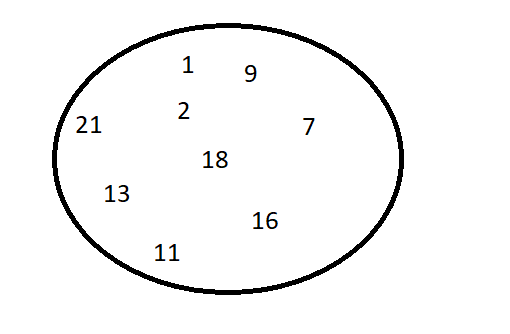
\includegraphics[width=0.45\linewidth]{Figuras/venn1}
	\caption{Diagrama De Venn.}
	\label{venn1}
\end{figure}

\textbf{Inclusão e subconjuntos}

\begin{definition}
	sejam $A$ e $B$ conjuntos. Dizemos que $A$ está contido em $B$ ($B$ contém $A$), denotado por $A \subset B$ ($ B \supset A $), se todo elemento de $A$ é elemento de $B$.
	
	Simbolicamente: $A \subset B \Leftrightarrow (\forall x, x \in A \implies x \in B)$.
	
	$A$ é subconjunto de $B$.
\end{definition}

\begin{figure}[h]
	\centering
	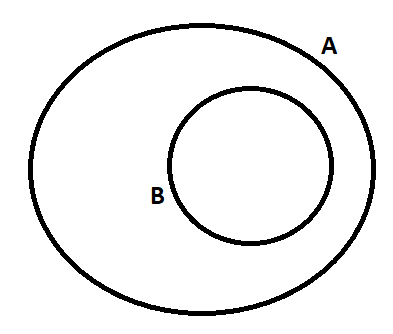
\includegraphics[width=0.3\linewidth]{Figuras/venn2}
	\caption{Diagrama De Venn para subconjunto.}
	\label{venn2}
\end{figure}


Por outro lado, se existe $x_0 \in A$ tal que $x_0 \notin B$, dizemos que $A$ não é subconjunto de $B$.

Simbolicamente: $A \not\subset B \Leftrightarrow (\exists x_0, x_0 \in A \text{ e } x_0 \notin B )$.
	
\begin{figure}[h]
	\centering
	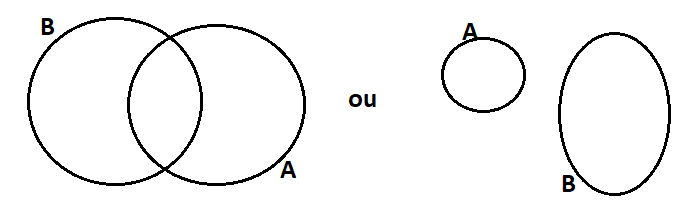
\includegraphics[width=0.5\linewidth]{Figuras/venn3}
	\caption{Diagrama De Venn para não subconjunto.}
	\label{venn3}
\end{figure}

\textbf{Propriedades da Inclusão:}Essas são as \textbf{relações de ordem}:
\begin{itemize}
	\item $\emptyset \subset A$ para todo $A$;
	\item $A \subset A$ para todo $A$ (reflexiva);
	\item $A \subseteq B$ e $B \subseteq A$ se, e somente se, $A=B$ (antissimétrica de inclusão);
	\item Se $A \subset B$ e $B \subset C$ então $A \subset C$ (transitividade).
\end{itemize}

Exemplo:
\begin{itemize}
	\item $1 \notin \{3, 4, \{1,2\}\}$ e $\{3, \{1,2\}\} \subset \{3, 4, \{1,2\}\}$
\end{itemize}

\textbf{União, interseção e diferença de conjuntos:} a união do conjunto $A$ com o conjunto $B$, denotada por $A \cup B$ é formada pelos elementos que estão em $A$ ou $B$.

\vspace{90pt}

\begin{center}
	\textcolor{red}{FIGURA 04 - DIAGRAMA DE VENN PARA UNIÃO DE CONJUNTOS}
\end{center}

A interseção do conjunto $A$ com o conjunto $B$, denotada por $A \cap B$, é o conjunto formado pelos elementos que estão em $A$ e $B$.

\vspace{90pt}
\begin{center}
	\textcolor{red}{FIGURA 05 - DIAGRAMA DE VENN PARA INTERSEÇÃO DE CONJUNTOS}	
\end{center}
	
Se $A \cap B = \emptyset$ dizemos que $A$ e $B$ são disjuntos.

\begin{proposition}
	$$ B \subset A \Leftrightarrow (A \cup B) = A$$
	$$ B \subset A \Leftrightarrow (A \cap B) = B$$
\end{proposition}

\textbf{Outras propriedades:}
\begin{enumerate}
	\item[Comutativa:] $A \cup B = B \cup A$ \\ $A \cap B = B \cap A$
	\item[Associativa:] $(A \cup B)\cup C = A \cup (B \cup C)$ \\ $(A \cap B) \cap C = A \cap (B \cap C)$
	\item[Distributiva:] $(A \cup B) \cap C = (A \cap C) \cup (B \cap C)$ \\ $(A \cap B)\cup C = (A \cup C) \cap (B \cup C)$
\end{enumerate}

\vspace{100pt}
\begin{center}
	\textcolor{red}{FIGURA 06 - DIAGRAMA DE VENN PARA DISTRIBUTIVA DE CONJUNTOS}	
\end{center}
	
A diferença entre $A$ e $B$, denotada por $A - B$, é o conjunto formado pelos elementos de $A$ que não pertencem a $B$.

\vspace{90pt}

\begin{center}
	\textcolor{red}{FIGURA 07 - DIAGRAMA DE VENN PARA SUBTRAÇÃO DE CONJUNTOS}	
\end{center}
	
Se $B \subset A$ então $\subset_{B}^{A} = A - B$ (complementar de $B$ em $A$).

Exemplo:
\begin{itemize}
	\item $\mathbb{Z} - \mathbb{N} = \{x \in \mathbb{Z} ; x \notin \mathbb{N} \}$  $=\{\dots, -3, -2, -1, 0 \}$
	\item $\mathbb{N} - \mathbb{Z} = \{x \in \mathbb{N}; x \notin \mathbb{Z} \} = \emptyset$
\end{itemize}	
	
\begin{proposition}
	$A \subset B$ se, e somente se, $A - B = \emptyset$.
\end{proposition}	
	
\textbf{Propriedades:}
\begin{itemize}
	\item [d:] $A \cap (B - C) = (A \cap B) - (A \cap C)$ \\ $A \cup (B - C) = (A \cup B) - (A \cup C)$
\end{itemize}

\vspace{90pt}

\begin{center}
	\textcolor{red}{FIGURA 08 - DIAGRAMA DE VENN PARA PROPRIEDADE $d$ DE CONJUNTOS}		
\end{center}
	
	
	
\subsection{Conjuntos Numéricos}
	
O conjunto $\mathbb{N}$	dos números naturais é caracterizado pelos axiomas de Peano.

\begin{enumerate}
	\item Todo número natural $n$ tem um sucessor $s(n)$, que ainda é um número natural, números diferentes têm sucessores diferentes.
	\item Existe um único número natural $1$ que não é sucessor de nenhum outro.
	\item Se um conjunto de números naturais contém o $1$ e contém também o sucessor de cada um de seus elementos, então esse conjunto contém todos os números naturais.
\end{enumerate}

No conjunto $\mathbb{N}$ dos números naturais são definidas duas operações fundamentais: adição e multiplicação, caracterizadas por:
\begin{multicols}{2}
\begin{itemize}
	\item $n+1 = s(n)$
	\item $n+s(m) = s(n+m)$
	\item $m \cdot 1 = m$
	\item $m \cdot s(n) = m \cdot n + m$
\end{itemize}
\end{multicols}
	
\textbf{Propriedades:}
\begin{enumerate}
	\item [Associativa:] $(m+n)+p = m+(n+p)$ \\ $m(np)=(mn)p$
	\item [Distributiva:] $m(n+p)=mn + mp$
	\item [Comutativa:] $m+n = n+m$ \\ $mn=nm$
	\item [Lei do Corte:] $n+m = p+m \implies n=p$ \\ $nm=pm \implies n=p$
\end{enumerate}
	
Outra propriedade importante de $\mathbb{N}$ é conhecida como {\it o Princípio da Boa Ordenação} que é todo subconjunto não-vazio $A \subseteq \mathbb{N}$ possui um menor elemento, isto é, um elemento $n_0 \in A$ tal que $n_o \leq n$ $\forall n \in A$.

\textbf{O conjunto $\mathbb{Z}$} dos números inteiros é definido por: $$\mathbb{Z} = \{ 0, \pm 1, \pm 2, \pm 3, \dots \}$$.


\textbf{O conjunto $\mathbb{Q}$} dos números racionais é formado pelas razões de inteiros: $$ \mathbb{Q} = \left\{ \frac{p}{q} ; p,q \in \mathbb{Z} \text{ e } q \neq 0 \right\}$$

Os racionais possuem expansões decimais que podem ser finitas, como $\frac{3}{4} = 0,750000\dots = 0,75\overline{0} = 0,75$, ou que se repetem indefinidamente (dízima periódica), como $\frac{23}{11} = 2,09090909\dots = 2,\overline{09}$.

Para encontrar a fração geratriz de um número com dízima periódica de período 1, multiplicamos e dividimos o número por $9$. Se o período é $2$, multiplicamos e dividimos por $99$. E assim por diante.

Exemplo:
\begin{multicols}{3}
\begin{itemize}
	\item $0,55555$ \\
	$\frac{5 - 0}{9} = \frac{5}{9} = 0,55555$
	\item $5,22222$ \\
	$\frac{52 - 5}{9} = \frac{47}{9} = 5,22222$
	\item $6,37777$ \\
	$\frac{637 - 63}{90} = \frac{574}{90} = 6,37777$
\end{itemize}
\end{multicols}

{\bf Exercício:} Qual o valor da expressão?
$$\left[(3^{0,3333333})^{27}+ 2^{2^1} - \sqrt[5]{239 + \sqrt[3]{\frac{448}{7}}}-(\sqrt[3]{3})^{3^3} \right]^{\sqrt[7]{92}}$$

Os números irracionais são os que não possuem expansão decimal sem dízima periódica, e assim não podem ser expressos por uma fração de inteiros, como $\sqrt{2}$, $\pi$, $\sin 1 ^{\circ}$, $\dots$

No cálculo quando falamos em ``número'', sem qualitativo, estaremos nos referindo ao conjunto dos números reais.

\textbf{O conjunto $\mathbb{R}$} dos números reais pode ser definido como o conjunto de todas as possíveis expansões decimais. Assim, um número real $a,d_{1}d_{2}d_{3}\dots$ pode ser representado por uma ``soma infinita'' de números racionais: $$a + \frac{d_1}{10} + \frac{d_2}{10^2} + \dots $$

\textbf{$\mathbb{R}$ é um corpo}, isto é, estão definidas em $\mathbb{R}$ duas operações: adição e multiplicação, que satisfazem as seguintes propriedades:
\begin{multicols}{2}
\begin{itemize}
	\item [Associativa:] $(x+y)+z = x+(y+z)$ \\ $(xy)z=x(yz)$
	\item [Comutativa:] $x+y=y+x$ \\ $xy=yx$
	\item [Distributiva:] $x(y+z) = xy + xz$
	\item [Elemento Neutro:] existem em $\mathbb{R}$ dois elementos distintos, $0$ e $1$, tais que: $x+0=x$ e $x \cdot 1= x$ para qualquer $x \in \mathbb{R}$
\end{itemize}
\end{multicols}

{\bf Inversos:} todo $x \in \mathbb{R}$ possui um {\it inverso aditivo} $(-x) \in \mathbb{R}$ tal que $x + (-x) = 0$ e se $x \neq 0$, existe também um {\it inverso multiplicativo} $x^{-1}$ tal que $x \cdot x^{-1} = 1$

A soma $x + (-y)$ é indicada por $x-y$ e é denominada {\bf diferença}.

O produto $x \cdot y^{-1} $ é indicado por $\frac{x}{y}$ e é denominado {\bf quociente}.

A divisão de $x$ por $y$ só faz sentido se $y \neq 0$. Podemos demonstrar outras propriedades como:

\begin{itemize}
	\item $xy=0 \implies x =0 \text{ ou } y=0$
	\item $x(-y)=(-x)y = -(xy)$
	\item $(-x)(-y)=xy$
	\item $x^2=y^2 \implies x = \pm y$
\end{itemize}

{\bf $\mathbb{R}$ é um corpo ordenado}, isto é, existe um subconjunto $\mathbb{R}_{+}^{*} \subset \mathbb{R}$ chamado o conjunto dos números reais positivos, que cumpre duas condições:
\begin{itemize}
	\item [p1:] $x,y \in \mathbb{R}_{+}^{*} \implies x+y \in \mathbb{R}_{+}^{*}$ e $xy \in \mathbb{R}_{+}^{*}$
	\item [p2:] Dado $x \in \mathbb{R}$, $x=0$ ou $x \in \mathbb{R}_{+}^{*}$ ou $(-x) \in \mathbb{R}_{+}^{*}$
\end{itemize}

Escreve-se $x<y$ e diz-se que $x$ é menor que $y$ se $y-x \in \mathbb{R}_{+}^{*}$. 

De {\bf p2}, segue que, dados $x,y \in \mathbb{R}$, $y-x=0$ ou $y-x \in \mathbb{R}_{+}^{*}$ ou $x-y \in \mathbb{R}_{+}^{*}$. Ou seja, $x=y$, $x>y$ ou $y>x$.

{\bf $\mathbb{R}$ é um corpo ordenado completo}, isto é, não possui espaços ``vazios'' na reta.


\subsubsection{A Reta Real}

Podemos usar as propriedades de ordem para representar geometricamente os números reais como pontos em uma reta numerada, onde ``a'' fica a esquerda de ``b'' se $a<b$.



\begin{figure}[h]
	\centering
	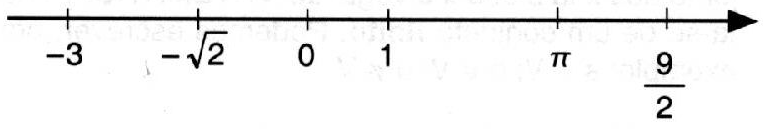
\includegraphics[width=0.5\linewidth]{Figuras/retareal11}
	\caption{Reta Real}
	\label{venn3}
\end{figure}

\textbf{Intervalos:} Um intervalo é um conjunto de números reais com a seguinte propriedade: dados dois números pertencentes ao intervalo, todos os números entre eles também pertencem ao intervalo.

São possíveis os seguintes intervalos:

\begin{table}[h!]
	\centering
	\begin{tabular}{|c|c|c|c|}
		\hline
		&	Notação			& Descrição do conjunto						 & Representação Geométrica \\
		\hline
		A	& $(a,b)$		& $\{ x \in \mathbb{R} ; a< x <b \} $		 & 	\\
		\hline
		B	& $[a,b]$		& $\{ x \in \mathbb{R} ; a\leq x \leq b \} $ & \\
		\hline
		C	& $[a,b)$		& $\{ x \in \mathbb{R} ; a\leq  x <b \} $	 & \\	
		\hline
		D	& $(a,b]$		& $\{ x \in \mathbb{R} ; a< x \leq b \} $	 & \\
		\hline
		E	& $(a, \infty)$	& $\{ x \in \mathbb{R} ; a< x < \infty \} $  & \\
		\hline
		F	& $[a,\infty)$	& $\{ x \in \mathbb{R} ; a \leq x <\infty \}$& \\
		\hline
		G	& $(- \infty,b)$& $\{ x \in \mathbb{R} ; - \infty < x <b \} $& \\
		\hline
		H	& $(- \infty, b]$& $\{ x \in \mathbb{R} ; -\infty< x \leq b \} $	 & \\
		\hline
		I	& $(- \infty, \infty)$ & $\mathbb{R}$ &	\\
		\hline
		J	& $[a,a]$		& $\{a\}$									 & \\
		\hline
	\end{tabular}
\end{table}

Um conjunto fechado contém toda a sua fronteira. Os intervalos $B,F,H,I$ e $J$ são fechados.

Um conjunto aberto só possui elementos internos do intervalo, não incluindo fronteira. Os intervalos $A,E,G$ e $I$ são abertos.

O intervalo $C$ é fechado à esquerda e aberto e à direita.

Os intervalos $A,B,C,D$ e $J$ são limitados.

Os intervalos $E,F,G,H$ e $I$ são ilimitados.

Os valores extremos do intervalo são chamados pontos de fronteira.

\textbf{Desigualdades:} Como um corpo ordenado, $\mathbb{R}$ possui as seguintes propriedades:
\begin{enumerate}
	\item $a<b$ e $b<c$ $\implies a<c$;
	\item $a<b$ $\implies a+c<b+c$ \\ $a<b$ $\implies a-c<b-c$
	\item $a<b$ e $c<d$ $\implies a+c<b+d$
	\item $a<b$ e $c>0$ $\implies ac<bc$ \\ $a<b$ e $c<0$ $\implies ac>bc$
	\item $a>0$ $\implies \frac{1}{a}>0$ \\ $a<0$ $\implies \frac{1}{a}<0$
	\item Se $a$ e $b$ são ambos positivos ou ambos negativos, então $a<b$ implica $\frac{1}{a} > \frac{1}{b}$. Se $a$ é negativo e $b$ positivo, então $\frac{1}{a} < \frac{1}{b}$
\end{enumerate}

\textbf{Exemplo:} Encontrar um intervalo em que $ \displaystyle -\frac{x}{3} < 2x + 1$

{\bf Solução:}

\begin{eqnarray*}
&  \displaystyle -\frac{x}{3} & < 2x + 1 \\ 
\implies & -x & < 3(2x + 1) \\
\implies & -x & < 6x + 3 \\
\implies & -x -6x & < 3 \\
\implies & -7x & < 3 \\
\implies & -x & < \frac{3}{7} \\
\implies & x & > - \frac{3}{7}
\end{eqnarray*}
{\it Resposta:} O conjunto solução da inequação $\displaystyle -\frac{x}{3} < 2x + 1$ é dado pelo intervalo real $\left(\displaystyle \frac{3}{7},+\infty\right)$.

\textbf{Valor Absoluto:} O valor absoluto de um número $x$ é a distância de $x$ a $0$ na reta real, dada por:

$$|x| = 
\begin{cases}
x, \text{  se } x \geq 0 \\
-x, \text{ se } x \leq 0
\end{cases}
$$

$$|x| = \sqrt{x^{2}} $$

\textbf{Exemplo:} Resolva $|2x - 5| = 3$

{\bf Solução:}

Por um lado:
\begin{eqnarray*}
	&  2x-5 & = 3 \\ 
	\implies & 2x & = 8 \\
	\implies & x & = 4 \\
\end{eqnarray*}

Por outro lado:
\begin{eqnarray*}
	&  2x-5 & = -3 \\ 
	\implies & 2x & = -3 + 5 \\
	\implies & x & = 1 \\
\end{eqnarray*}

{\it Resposta:} O conjunto solução é $\{1,4\}$.

\textbf{Exemplo:} Resolva $|x - 5| < 2$

{\bf Solução:}

Se: $x - 5 \geq 0$, então: $x \geq 5$ e assim: $x - 5 < 2 \implies x < 7$

Se: $x - 5 < 0$, então: $x < 5$ e assim: $-x +5 < 2 \implies x > 3$

{\it Resposta:} $S:\{x \in \mathbb{R};3 < x < 7\}$

\textbf{Exemplo:} Resolva $|3x + 2| \geq 4$

{\bf Solução:}

Se $3x + 2 \geq 0$, então $x \geq \displaystyle -\frac{2}{3}$ e assim: $3x + 2 \geq 4 \implies x \geq \displaystyle \frac{2}{3}$. 

Portanto, o conjunto solução $01$ será: $S_1 = \left\{ x \in \mathbb{R}; x \geq \displaystyle \frac{2}{3} \right\}$

Se $3x + 2 < 0$, então $x < \displaystyle - \frac{2}{3}$ e assim: $-3x - 2 \geq 4 \implies x \leq -2$

Portanto, o conjunto solução $02$ será: $S_2 = \left\{ x \in \mathbb{R}; x \leq -2 \right\}$

Realizando a união das soluções, tem-se: $S_{final} = \left\{ x \in \mathbb{R}; x \leq -2 \text{ ou } x \geq \displaystyle - \frac{2}{3} \right\}$ em outras palavras: $x \in \left( -\infty,-2 \right] \displaystyle \cup \left[\frac{2}{3},+ \infty \right)$

{\bf Algumas propriedades:}
\begin{enumerate}
	\item $|x| = a \Leftrightarrow x = \pm a$
	\item $|x| < a \Leftrightarrow -a < x < a$
	\item $|x| > a \Leftrightarrow x>a$ ou $x<a$
	\item $|-a| = |a|$
	\item $|ab|=|a|.|b|$
	\item $|\frac{a}{b}| = \frac{|a|}{|b|}$
	\item $|a^{n}| = |a|^{n}$
	\item $|a+b| \leq |a| + |b|$ Desigualdade Triangular
\end{enumerate}

\textbf{Exercícios}

\subsubsection{Equações de 1º Grau}

São expressões do tipo $ax+b=0$, com $a \neq 0$, onde $a$ e $b$ são coeficientes da equação e $x$ é a incógnita.

O valor que se substituído na equação e torna a sentença verdadeira é chamado de {\it raiz da equação}.

A equação do primeiro grau pode não ter solução em $\mathbb{N}$ ou $\mathbb{Z}$, mas sempre possui uma solução em $\mathbb{Q}$ ou $\mathbb{R}$.

Observe:

\begin{eqnarray*}
	&  ax + b & = 0 \\
	\implies & ax + b - b & = -b \\
	\implies & ax & = -b \\
	\implies & \displaystyle \frac{ax}{a} & = \displaystyle - \frac{b}{a}\\
	\implies & x & = \displaystyle - \frac{b}{a}
\end{eqnarray*}

\subsubsection{Equações de 2º Grau}

São expressões do tipo $ax^{2} + bx + c = 0$, com $a \neq 0$, onde $a,b$ e $c$ são coeficientes e $x$ é a incógnita. Nem sempre possui raízes reais, mas possui uma ou duas raízes em $\mathbb{C}$. Vejamos:

\begin{eqnarray*}
	&  ax^2 + bx + c & = 0 \\
	\implies & a\left( x^2 + \displaystyle \frac{bx}{a} + \displaystyle \frac{c}{a} \right) & = 0 \\
	\implies & x^2 + \displaystyle \frac{bx}{a} + \displaystyle \frac{c}{a} & = 0 \\
	\implies & x^2 + \displaystyle \frac{bx}{a} & = - \displaystyle \frac{c}{a}\\
	\implies & x^2 + \displaystyle \frac{bx}{a} + \displaystyle \frac{b^2}{4a^2} & = \displaystyle - \frac{c}{a} + \displaystyle \frac{b^2}{4a^2} \text{ * OBS1 abaixo *} \\
	\implies & \left( x + \displaystyle \frac{b}{2a} \right)^2 & = \displaystyle - \frac{c}{a} + \displaystyle \frac{b^2}{4a^2} \\
	\implies & \left| x + \displaystyle \frac{b}{2a} \right| & = \displaystyle \sqrt{\displaystyle \frac{b^2}{4a^2} - \displaystyle \frac{c}{a}} \\
	\implies & x + \displaystyle \frac{b}{2a} & \pm \displaystyle \sqrt{\displaystyle \frac{b^2 - 4ac}{4a^2}}\\
	\implies & x & = - \displaystyle \frac{b}{2a} \pm \displaystyle \frac{\displaystyle \sqrt{b^2 - 4ac}}{2a} \\
\end{eqnarray*}

Chegando na {\bf Fórmula Geral de Resolução da Equação de 2$^\circ$ Grau:}

\begin{equation}
x = \displaystyle \frac{-b \pm \displaystyle \sqrt{b^2 - 4ac}}{2ac}
\end{equation}

{\bf * OBS1 *}

$$(x+k)^2 = x^2 + 2kx + k^2$$
$$\implies 2k = \displaystyle \frac{b}{a} \text{ , } k = \displaystyle \frac{b}{2a} \text{ , } k^2 = \displaystyle \frac{b^2}{4a^2}$$

A existência de raízes reais dependerá do valor de $\Delta = b^2 - 4ac$. Suponha, então que $\Delta \geq 0 $, assim:
$$x_1 = \displaystyle \frac{-b + \displaystyle \sqrt{b^2 - 4ac}}{2ac}$$
$$x_2 = \displaystyle \frac{-b - \displaystyle \sqrt{b^2 - 4ac}}{2ac}$$

E assim:

$$ a(x - x_1)(x - x_2)  = ax^2 +bx + c = 0 \text{ * VERIFIQUE!!! *} $$

Mas note que:

$$a(x - x_1)(x - x_2) = a(x^2 + (-x_1 - x_2)x + x_1 x_2)$$

Como:

$$a\left[x^2 + (-x_1-x_2)x + x_1 x_2 \right] = a\left[ x^2 + \frac{b}{a} + \frac{c}{a} \right]$$

Temos as {\bf Relações de Girard}:
$$\displaystyle \frac{b}{a} = -x_1 - x_2 \implies - \displaystyle \frac{b}{a} = x_1 + x_2$$
$$\displaystyle \frac{c}{a} = x_1 x_2$$


\subsubsection{Inequações de 2º Grau}

\textbf{Exemplo 01:}Resolva a desigualdade $x^{2} - 5x + 6 \leq 0$

{\bf Solução:}

Fatorando o lado esquerdo da inequação: $a(x-x_1)(x-x_2) \leq 0$ 
$$(x-2)(x-3) \leq 0$$

Avaliando o sinal nos intervalos:

Se $x \in (-\infty,2) \implies x < 2$, logo:
$$x-2<0 \land x-3 < 0 $$

Se $x \in (2,3) \implies 2<x<3$, logo:
$$x-2 > 0 \land x-3 < 3$$

Se $x \in (3, \infty) \implies x > 3$, logo:
$$x - 2 > \land x - 3>0$$

Assim temos a tabela:
\begin{table}[h]
	\centering
	\begin{tabular}{|c|c|c|c|}
		\hline
		Intervalo \ Fator	&	$x-2$	&	$x-3$	&	$(x-2)(x-3)$ \\
		\hline
		$x<2$				&	-		&	-		&	+	\\
		\hline
		$2<x<3$				&	+		&	-		&	-	\\
		\hline
		$x>3$				&	+		&	+		&	+	\\
		\hline
	\end{tabular}
\end{table}
	
\textbf{Modo Visual:} Considerando a parábola $y=x^{2}-5x+6$, que possui concavidade voltada para cima, podemos ver que $y$ possui valores negativos em $(2,3)$:
\begin{figure}[h!]
	\centering
	\begin{tikzpicture}[line cap=round,line join=round,>=triangle 45,x=1cm,y=1cm]
	\begin{axis}[
	x=1cm,y=1cm,
	axis lines=middle,
	ymajorgrids=true,
	xmajorgrids=true,
	xmin=-0.7111076040956626,
	xmax=7.037428115508905,
	ymin=-2.3583189639033857,
	ymax=2.5546348694497114,
	xtick={-0.5,0,...,7},
	ytick={-2,-1.5,...,2.5},]
	\clip(-0.7111076040956626,-2.3583189639033857) rectangle (7.037428115508905,2.5546348694497114);
	\draw [samples=50,rotate around={0:(2.5,-0.25)},xshift=2.5cm,yshift=-0.25cm,line width=2pt,domain=-4:4)] plot (\x,{(\x)^2/2/0.5});
	\begin{scriptsize}
	\draw[color=black] (1.6436582231827345,0.8255463496811495) node {$f$};
	\end{scriptsize}
	\end{axis}
	\end{tikzpicture}
	\caption{Gráfico de $y=x^{2}-5x+6$.}
\end{figure}


\textbf{Exemplo 2:} $x^{3} + 3x^{2} > 4x$

{\bf Solução:}

\begin{eqnarray*}
	&  x^3 + 3x^2 - 4x & > 0 \\
	\implies & x(x^2 + 3x - 4) & > 0 \\
	\implies & x_1 = 1 \land x_2 & = -4 \\
	\implies & (x-0)(x-1)(x+4) & > 0
\end{eqnarray*}


\begin{table}[h]
	\centering
	\begin{tabular}{|c|c|c|c|c|}
		\hline
		Intervalo \ Fator	&	$x$	&	$x-1$	&	$x+4$	&	$x(x-1)(x+4)$ \\
		\hline
		$x<-4$				&	-		&	-		&	-	&	-	\\
		\hline
		$-4<x<0$			&	-		&	-		&	+	&	+	\\
		\hline
		$0<x<1$				&	+		&	-		&	+	&	-	\\
		\hline
		$x>1$				&	+		&	+		&	+	&	+	\\
		\hline
	\end{tabular}
\end{table}

O conjunto solução será: $S= \{ x\in \mathbb{R} ; -4 < x < 0 \text{ ou } x > 1 \}$ $=$ $(-4,0) \cup (1,\infty)$.

\textbf{Exercícios}

\subsubsection{Teorema Fundamental da Álgebra}

Todo polinômio de grau $n$, $n \geq 1$ admite ao menos uma raiz complexa.

\subsubsection{Teorema da Decomposição}

Seja $p(x)$ um polinômio de grau $n$, $n \geq 1$, dado por: $$p(x) = a_nx^n+a_{n-1}x^{n-1}+\dots+a_1x+a_0$$ com $a_n \neq 0$. Então, $p(x)$ pode ser decomposto em $n$ fatores do $1º$ grau sob a forma:
$$p(x) = a_n(x-r_1)(x-r_2)\dots(x-r_n)$$
em que $r_1, r_2, \dots, r_n$ são as raízes de $p(x)$ e $a_n$ é o coeficiente dominantes de $p(x)$.

\textbf{Relações de Girard}

Sejam $r_1,r_2$ e $r_3$ as raízes da equação $ax^{3}+bx^{2}+cx+d=0$, com $a \neq 0$. Temos:

{\it Verifique!!!!!}


\textbf{Exemplo:} Resolva $x^3-9x^2+26x-24=0$, sabendo que as raízes são inteiras.

{\bf Solução:}

$$\begin{cases}
	r_1+r_2+r_3 = 9 \\
	r_1r_2r_3 = 24
\end{cases}$$

Logo, $r_1 = 2$, $r_2 = 3$ e $r_3 = 4$.

\subsubsection{Divisão de Polinômios}

Seja $f(x) = a_0x^n+a_1x^{n-1}+\dots+a_{n-1}x+a_n$ e $g(x)=x-a$. Se $f(a)=0$, então existe $q(x)=q_0x^{n-1}+q_1x^{n-2}+\dots+q_{n-2}x+q_{n-1}$ tal que $q(x).g(x)=f(x)$.

\textbf{Exemplo:} Considere $f(x)=x^3-9x^2+26x-24$ e $g(x)=x-2$.

\vspace{200pt}

\textbf{Teorema das Raízes Racionais} Se $a_nx^n+a_{n-1}x^{n-1}+\dots+a_1x+a_0 = 0$ é uma equação polinomial com coeficientes inteiros, com $a_n \neq 0$ e o número racional $\frac{p}{q}$, com $p$ e $q$ primos entre si, é raiz dessa equação, então $p$ é divisor de $a_0$ e $q$ é divisor de $a_n$.

\textbf{Exemplo:} Resolva a equação $3x^3-7x^2+8x-2=0$, sabendo que possui raízes racionais.

{\bf Solução:}

$p$ é divisor de $(-2) \implies p \in \{ -1,1,-2,2 \}$

$q$ é divisor de $(3) \implies q \in \{ -1,1,-3,3 \}$

Os candidatos as raízes são $\frac{p}{q}$, então: $\left\{1,-1, \displaystyle \frac{2}{3}, -\displaystyle \frac{2}{3},2,-2,\displaystyle \frac{1}{3}, -\displaystyle \frac{1}{3} \right\}$

Fazendo as verificações, temos que $\displaystyle \frac{1}{3}$ é a raiz da equação, logo basta dividir por $\left( x - \displaystyle \frac{1}{3} \right) $ para obter uma nova equação e determinar as raízes restantes.

\textbf{Exercícios}

\subsubsection{Produto Cartesiano}

Sejam dois conjuntos $A$ e $B$ não vazios. Define-se como {\it produto cartesiano} $A$ por $B$ o conjunto $A \times B$ de todos os pares ordenados $(x,y)$ onde o $x \in A$ e $y \in B$.

\vspace{130pt}
{\bf IMAGEM IMAGEM }
$$A \times B = \{ (1,4), (1,5), (2,4), (2,5), (3,4), (3,5)  \}$$

\textbf{Exemplo:} Determine $A \times B$ se:
\begin{itemize}
	\item $A = \{1,2,3\}$ \\ $B = \{4,5\}$
	\item $A = \{ x \in \mathbb{R} ; -1 \leq x \leq 2 \}$ \\ $B=\{3\}$
	\item $A = \{ x \in \mathbb{R} ; -2 \leq x \leq 1 \}$ \\ $B=\{y \in \mathbb{R}; -1 \leq y \leq 3\}$
\end{itemize}

{\bf Solução:}\\
$A \times B = \{ (1,4), (1,5), (2,4), (2,5), (3,4), (3,5)  \}$\\
$A \times B = \{ (x,3) \in \mathbb{R}; -1\leq x \leq 2  \}$\\
$A \times B = \{ (x,y) \in\mathbb{R}^2; -2 \leq x \leq 1 \land -1 \leq y \leq 3  \}$


\newpage

\textbf{Relação Binária}

Uma relação qualquer que relaciona qualquer subconjunto do produto cartesiano $A \times B$, ou seja, $R: A \rightarrow B$, bem como $R \subset A \times B$.

\textbf{Exemplo:} Seja $A=\{1,2,3\}$ e $B=\{4,5\}$. Determine $R_1$ onde $x=1$ e $R_2$ onde $y=4$.
	
{\bf Solução:}

$A \times B = \{ (1,4), (1,5), (2,4), (2,5), (3,4), (3,5)  \}$

$R_1 = \{ (1,4), (1,5) \}$ Relação $x=1$.

$R_2 = \{ (1,4), (2,4), (3,4)  \}$ Relação $y = 4$.

\newpage
\begin{snugshade}
	\section{Funções Reais de uma Variável Real}
\end{snugshade}	
	
Sejam $D$ e $Y$ conjuntos não-degenerados. Uma função $f:D \rightarrow Y$ é uma regra que associa, a cada elemento $x \in D$, um único elemento $f(x) \in Y$.

\begin{definition}[Função]
	É uma relação em que todos os elementos $x$ do conjunto $A$, se relacionam uma {\bf única} vez com os elementos $y$ do conjunto $B$, ou seja, $f: A \rightarrow B$, ou ainda, $(f): \mathbb{R} \rightarrow \mathbb{R}$, ou simplesmente $(f): X\rightarrow Y = f(x)$, na prática escrevemos $y = f(x)$.
	
	Uma função pode ser representada na forma:
	\begin{enumerate}
		\item Verbalmente, através de palavras;
		\item Numericamente, através de tabelas;
		\item Visualmente, através de gráficos;
		\item Matematicamente, através da lei da correspondência, $y = f(x)$.
	\end{enumerate}
\end{definition}

O conjunto $D$ é denominado domínio da função. O conjunto $Y$ é denominado contra-domínio. A imagem da função $f$ é o conjunto formado por todos os pontos $y \in Y$ tais que existe um $x_0 \in D$ com $f(x_0) = y$. Note que $Im(f) \subset Y$, mas não necessariamente a imagem possui todos os elementos do contra-domínio.

\textbf{Exemplo: } Um carro se move à velocidade constante de $80$km/h. A cada hora de viagem, a distância percorrida desde o ponto de partida é marcada como na tabela abaixo:
\begin{table}[h]
	\centering
	\begin{tabular}{|c|c|}
		\hline
		t(horas)	&	d(quilômetros) \\
		\hline
		$1$			&	$80$	\\
		\hline
		$2$			&	$160$	\\
		\hline
		$3$			&	$240$	\\
		\hline
		$4$			&	$320$	\\
		\hline
		$\vdots$		&	$\vdots$	\\
		\hline	
	\end{tabular}
\end{table}
	
Podemos definir $f:\mathbb{N} \rightarrow \mathbb{Z}$ por: $f(t) \in \mathbb{Z}$ é a quantidade de quilômetros percorridos após $t$ horas.

Observe que o domínio desta função é $\mathbb{N}$, contra-domínio é $\mathbb{Z}$ e a imagem é $\{80,160,240,320,\dots\}$.

Podemos representar uma função através de setas no diagrama de Venn-Euler.


\vspace{90pt}

\begin{center}
	\textcolor{red}{FIGURA 10 - DIAGRAMA DE VENN PARA A FUNÇÃO}
\end{center}
	
Quando uma função está definida no conjunto dos números reais, considera-se que o domínio seja o maior conjunto de valores de $x$ para os quais $f(x)$ existe (em $\mathbb{R}$).

\textbf{Exemplo: (tabela)}	

\begin{table}[h!]
	\centering
	\begin{tabular}{|c|c|c|}
		\hline
		Função		&	Domínio					&	Imagem	\\
		\hline
		$f(x)=x^2$	&	$(-\infty, \infty)$		&	$[0, \infty)$	\\
		\hline
		$y=\frac{1}{x}$	&	$(-\infty,0) \cup (0,\infty)$	& $(-\infty,0) \cup (0,\infty)$	\\
		\hline
		$\sqrt{x}$	&	$[0,\infty)$			&	$[0,\infty)$	\\
		\hline
		$y=\sqrt{4-x}$	&	$(-\infty,4]$		&	$[0,\infty)$	\\
		\hline
		$y=\sqrt{1-x^2}$&	$[-1,1]$			&	$[0,1]$	\\
		\hline		
	\end{tabular}
\end{table}
	
\textbf{Exercícios: }Determine o domínio das seguintes funções:
\begin{enumerate}

\item $f(x) = \frac{1}{x}$

{\bf Solução:}

Condição de Existência: $x \neq 0$

Logo, $D(f(x)) = \{ x \in \mathbb{R}; x \neq 0\}$

\item $f(x) = \sqrt{x-2}$

{\bf Solução:}

Condição de Existência: $x - 2 \geq 0 \implies x \geq 2$

Logo, $D(f(x)) = \{ x \in \mathbb{R}; x \geq 2 \}$

\item $f(x) = \sqrt{x^2 - 7x + 10}$

{\bf Solução:}

Condição de Existência: $x^2 - 7x + 10 \geq 0$

Suas raízes são: $2$ e $5$. Através da análise das raízes, conclui-se:

Logo, $D(f(x)) = \{ x \in \mathbb{R}; x \leq 2 \cup x \geq 5 \}$ ou ainda $D(f(x)) = (-\infty,2]\cup[5,\infty)$

\item $f(x) = \frac{1}{x^2 - 9}$

{\bf Solução:}

Condição de Existência: $x^2 - 9 \neq 0 \implies x \neq \pm 3$.

Logo, $D(f(x)) = \{ x \in \mathbb{R}; x \neq \pm 3 \}$

\item $f(x) = |x|$

{\bf Solução:}

$D(f(x)) = \mathbb{R}$

\item $f(x) = \ln(2x - 4)$

{\bf Solução:}

Condição de Existência: $2x - 4 \geq 0 \implies x \geq 2$.

Logo, $D(f(x)) = \{ x \in \mathbb{R}; x \geq 2 \}$

\item $f(x) = \sin(x)$

{\bf Solução:}

$D(f(x)) = \mathbb{R}$

\item $f(x) = \arcsin(x)$

{\bf Solução:}

$D(f(x)) = \{ x \in \mathbb{R}; -1\leq x \leq 1 \}$

\item $f(x) = \frac{1}{\sqrt{x^2 - 16}}$

{\bf Solução:}

Condição de Existência: $x^2 - 16 \geq 0 \implies x \geq \pm 4$.

Analisando as raízes, obtém-se:

$D(f(x)) = \{ x \in \mathbb{R}; x < -4 \lor x > 4 \}$

\end{enumerate}
O gráfico de uma função é definido pelo conjunto dos pares ordenados $(x,f(x))$, ou seja: $$G(f)=\{(x,f(x));x \in D\}$$	
	
\textbf{Exemplo: }o gráfico da função $f(x)=x+2$ é o conjunto dos pontos com coordenadas $(x,y)$ para os quais $y=x+2$.	

\begin{figure}[h]
	\centering
	\begin{tikzpicture}
		\begin{axis}
			[
			axis x line=center,
			axis y line=center,
			xtick={-10,-9,...,10},
			ytick={-10,-9,...,10},
			xlabel={$x$},
			ylabel={$y$},
			xlabel style={below right},
			ylabel style={above left},
			xmin=-10.5,
			xmax=10.5,
			ymin=-10.5,
			ymax=10.5,
			width=15cm
			]
			\addplot
			[
					domain =-9:9,
					color=red,
			]
			{x + 2};
			\addlegendentry {$y = x + 2$}
		\end{axis}
	\end{tikzpicture}
	\caption{Gráfico da função $y = x + 2$.}
\end{figure}


Nem toda linha no plano cartesiano representa uma função. Um gráfico é um conjunto de pares ordenados por uma função, nem todo conjunto forma um gráfico, mas sim uma representação gráfica. Por exemplo, o conjunto $\{(x,y); x^2 + y^2 = 1\}$ forma uma representação gráfica.

\vspace{90pt}

\begin{center}
	\textcolor{red}{FIGURA 11 - REPRESENTAÇÃO GRÁFICA DE $\{(x,y); x^2 + y^2 = 1\}$}
\end{center}


\subsection{Funções Definidas por Partes}

Uma função pode ser descrita por fórmulas diferentes a partes diferentes de seu domínio. Por exemplo, a função valor absoluto.

$$|x| = 
\begin{cases}
x, \text{  se } x \geq 0 \\
-x, \text{ se } x < 0
\end{cases}
$$

Outro exemplo: uma função pode ser descrita por fórmulas diferentes  a partes diferentes do seu domínio. Por exemplo:

\vspace{90pt}
.
\begin{center}
	\textcolor{red}{FIGURA 12 - REPRESENTAÇÃO GRÁFICA DE $f(x) = k$ se $k \leq x < k+1$}
\end{center}


\subsection{Simetrias}

Uma função $y=f(x)$ é dita:
\begin{itemize}
	\item par, se $f(-x) = f(x)$, $\forall x \in D$; \\ Simetria em relação ao eixo $y$.
	\item ímpar, se $f(-x) = -f(x)$, $\forall x \in D$. \\ Simetria em relação à origem.
\end{itemize}

\textbf{Exemplo: } $f(x)=x^2$ é uma função par e $g(x) = x^3$ é uma função ímpar.

\begin{figure}[h]
	\centering
	\begin{tikzpicture}
	\begin{axis}
	[
	axis x line=center,
	axis y line=center,
	xtick={-10,-9,...,10},
	ytick={-10,-9,...,10},
	xlabel={$x$},
	ylabel={$y$},
	xlabel style={below right},
	ylabel style={above left},
	xmin=-10.5,
	xmax=10.5,
	ymin=-10.5,
	ymax=10.5,
	width=10cm
	]
	\addplot
	[
	domain =-9:9,
	color=red,
	]
	{x^2};
	\addlegendentry {$y = x^2$}
	\end{axis}
	\end{tikzpicture}
	\caption{Gráfico da função $y = x^2$.}
\end{figure}

\begin{figure}[h]
	\centering
	\begin{tikzpicture}
	\begin{axis}
	[
	axis x line=center,
	axis y line=center,
	xtick={-10,-9,...,10},
	ytick={-10,-9,...,10},
	xlabel={$x$},
	ylabel={$y$},
	xlabel style={below right},
	ylabel style={above left},
	xmin=-10.5,
	xmax=10.5,
	ymin=-10.5,
	ymax=10.5,
	width=10cm
	]
	\addplot
	[
	domain =-9:9,
	color=red,
	]
	{x^3};
	\addlegendentry {$y = x^3$}
	\end{axis}
	\end{tikzpicture}
	\caption{Gráfico da função $y = x^3$.}
\end{figure}


De fato, $f(-x) = (-x)^2 = x^2 = f(x)$ e $g(-x) = (-x)^3 = (-x)(x)^2 = -x^3=-g(x)$

\subsection{Funções Monótonas}
Uma função $f:D \rightarrow \mathbb{R}$, com $D \subset \mathbb{R}$, chama-se:
\begin{itemize}
	\item não-decrescente, se $x<y \Rightarrow f(x) \leq f(y)$;
	\item não-crescente, se $x<y \Rightarrow f(x) \geq f(y)$;
	\item crescente, se $x<y \Rightarrow f(x) < f(y)$;
	\item decrescente, se $x<y \Rightarrow f(x) > f(y)$.
\end{itemize}

\textbf{Exemplo :}
\begin{enumerate}
	\item A função $\sqrt{x}$ é crescente em todo domínio $[0, \infty)$;
	\item A função $f(x) = 1 - x$ é decrescente em $\mathbb{R}$;
	\item A função $f(x) = 5$ é não-decrescente e não-crescente em $\mathbb{R}$.
\end{enumerate}


\subsection{Composição de Funções}

Sejam $A$, $B$ e $C$ conjuntos e sejam as funções $f:A \rightarrow B$ e $g: B \rightarrow C$. A função $ g \circ f : A \rightarrow C$ é definida por:
$$(g \circ f)(x) = g(f(x))$$

Note que $g \circ f$ costuma ser diferente de $ f \circ g$.

\textbf{Exemplo: } Tome $f(x) = \sqrt{x}$ e $g(x) = x + 1$.

{\bf Solução:}

$g \circ f = g(f(x)) = \sqrt{x}+1$ e $D(g \circ f) = [0,\infty)$

$f \circ g = f(g(x)) = \sqrt{x+1}$ e $D(f \circ g) = [-1,\infty)$

Uma função $f:D \rightarrow Y$ é dita {\it injetora} se $f(x_1) \neq f(x_2)$ sempre que $x_1 \neq x_2$ em $D$. Em outras palavras, $f$ é injetora se $f(x_1) = f(x_2)$ implica em $x_1 = x_2$. Para cada $y = f(x)$ só há um $x$ que satisfaça.


\vspace{150pt}
.
\begin{center}
	\textcolor{red}{FIGURA 13 - REPRESENTAÇÃO GRÁFICA DE FUNÇÃO INJETORA}
\end{center}

Uma função $f:D \rightarrow Y$ é dita {\it sobrejetora} se, para cada $y \in Y$, existe $x \in D$ tal que $f(x) = y$. Ou seja, $f$ é sobrejetora se $Im(f) = Y$.

Observe que se restringirmos o contra-domínio à imagem, ou seja, tomarmos $f: D \rightarrow Im(f)$ pela mesma lei de formação, teremos uma função sobrejetora.

\textbf{Exemplo: } $f: \mathbb{R} \rightarrow \mathbb{R}$ dada por $f(x) = x^2$ não é sobrejetora, mas $f: \mathbb{R} \rightarrow [0, \infty)$ dada por $f(x)=x^2$ é sobrejetora.

Uma função injetora e sobrejetora é dita {\it bijetora}.

Se $f: D \rightarrow Y$ é bijetora, então, para cada $y \in Y$, existe um único $x \in D$ tal que $f(x)=y$.

Assim, podemos definir $f^{-1}:Y \rightarrow D$ por 
$$f^{-1}(y) = x \text{ se } f(x) = y$$

Temos que:

$f \circ f^{-1}(y) = f(f^{-1}(y)) = f(x) = y$ 

$f^{-1} \circ f(x) = f^{-1}(f(x)) = f^{-1}(y) = x $

\textbf{Exemplo: } Determinar a inversa de $y = f(x) = \displaystyle \frac{1}{2}x + 1$

{\bf Solução:}

\begin{eqnarray*}
	&  y & = \displaystyle \frac{1}{2}x + 1  \\
	\implies & x & = \displaystyle \frac{1}{2}y + 1 \\
	\implies & x - 1 & = \displaystyle \frac{1}{2}y \\
	\implies & 2x - 2 & = y 
\end{eqnarray*}

Logo, $f^{-1}(x) = 2x - 2$



\begin{center}
	\textcolor{red}{FIGURA 13.1 - REPRESENTAÇÃO GRÁFICA (DIAG. VENN) DOS TIPOS DE FUNÇÕES}
\end{center}

\subsection{Operações com Funções}

Se $f$ e $g$ são funções, com domínios $D(f)$ e $D(g)$, respectivamente, então podemos definir em $D(f) \cap D(g)$ as funções:
\begin{eqnarray*}
(f \pm g)(x) = f(x) \pm g(x) \\
(f \cdot g)(x) = f(x) \cdot g(x) \\
\text{E para os pontos em que $g(x) \neq 0$: } \\
\frac{f}{g}(x) = \frac{f(x)}{g(x)} \text{ com $D(\frac{f}{g}) = D(f) \cap D(g)$ ; $g(x) \neq 0$}
\end{eqnarray*}
Funções também podem ser multiplicadas por constantes: $$(cf)(x) = c \cdot f(x)$$

\subsection{Translação}
Se $k > 0$, $y = f(x) + k$ translada o gráfico de $f$, $k$ unidades para cima e $y = f(x) - k$ translada $k$ unidades para baixo.

Se $h>0$, $y = f(x+h)$ translada o gráfico de $f$, $h$ unidades para a esquerda e $f(x-h)$ translada $h$ unidades para a direita.

\subsection{Reflexão e mudança de escala}

\begin{itemize}
	\item $y = -f(x)$ reflete o gráfico de $f$ em torno do eixo $x$;
	\item $y = f(-x)$ reflete o gráfico de $f$ em torno do eixo $y$;
	\item Se $c>1$, $y = f(cx)$ alonga verticalmente o gráfico de $f$;
	\item Se $0<c<1$, $y=f(cx)$ alonga horizontalmente o gráfico de $f$.
\end{itemize}

\subsection{Principais Funções Elementares}

\subsubsection{Função Polinomial}

$$f(x) = a_0+a_1x+a_2x^2+\dots+a_nx^n$$

Em especial tem-se a {\it função nula} $g(x) \equiv =$ e a {\it função constante} $f(x) = a_0$

\begin{figure}[h]
	\centering
	\begin{tikzpicture}
	\begin{axis}
	[
	axis x line=center,
	axis y line=center,
	xtick={-10,-9,...,10},
	ytick={-10,-9,...,10},
	xlabel={$x$},
	ylabel={$y$},
	xlabel style={below right},
	ylabel style={above left},
	xmin=-5,
	xmax=5,
	ymin=-3,
	ymax=5,
	width=10cm
	]
	\addplot
	[
	domain =-9:9,
	color=red,
	]
	{3};
	\addlegendentry {$y = 3$}
	\end{axis}
	\end{tikzpicture}
	\caption{Gráfico da função $y = 3$.}
\end{figure}

Tem-se a {\it função afim (ou linear)} quando $f(x) = ax+b$

\begin{figure}[h!]
	\centering
	 \definecolor{qqwuqq}{rgb}{0,0.39215686274509803,0}
	 \begin{tikzpicture}[line cap=round,line join=round,>=triangle 45,x=2cm,y=2cm]
	 \begin{axis}[
	 x=2cm,y=2cm,
	 axis lines=middle,
	 xmin=-3.6576470424178473,
	 xmax=4.090888677186721,
	 ymin=-1.8528456711368184,
	 ymax=3.0601081622162782,
	 xtick={-3.5,-3,...,4},
	 ytick={-1.5,-1,...,3},]
	 \clip(-3.6576470424178473,-1.8528456711368184) rectangle (4.090888677186721,3.0601081622162782);
	 \draw[line width=2pt,color=qqwuqq,smooth,samples=100,domain=-3.6576470424178473:4.090888677186721] plot(\x,{(\x)+1});
	 \draw (0.047102335054185665,1.0628722249435012) node[anchor=north west] {-b};
	 \draw (-1.1980879715171133,0.17521180837782244) node[anchor=north west] {-b/a};
	 \begin{scriptsize}
	 \draw[color=qqwuqq] (-2.7576580089554232,-1.7511345817386676) node {$f$};
	 \end{scriptsize}
	 \end{axis}
	 \end{tikzpicture}
	 \caption{Função Afim}
\end{figure}

Onde $a \neq 0$ e $a$ é o coeficiente angular, $b$ é o coeficiente linear. O gráfico é uma reta que pode ser crescente $(a>0)$ ou decrescente $(a<0)$.

\textbf{Função Quadrática ou $2^{\circ}$ Grau}

A função $y = ax^2+ bx + c$ com $a \neq 0$ e $a,b$ e $c$ são constantes é denominada função quadrática. O gráfico é uma parábola com simetria perpendicular ao eixo $x$.

Os vértices são:
$$V_x = - \frac{b}{2a} $$
$$V_y = - \frac{\Delta}{4a} $$

\vspace{150pt}
\begin{center}
	\textcolor{red}{FIGURA 13 - REPRESENTAÇÃO GRÁFICA DE FUNÇÃO QUADRÁTICA}
\end{center}

\subsubsection{Função Racional}

$f(x) = \frac{p(x)}{q(x)}$, onde $p$ e $q$ são funções polinomiais. O domínio de $f$ é $\{x \in \mathbb{R}; q(x) \neq 0 \}$

\begin{figure}[h!]
		\centering
		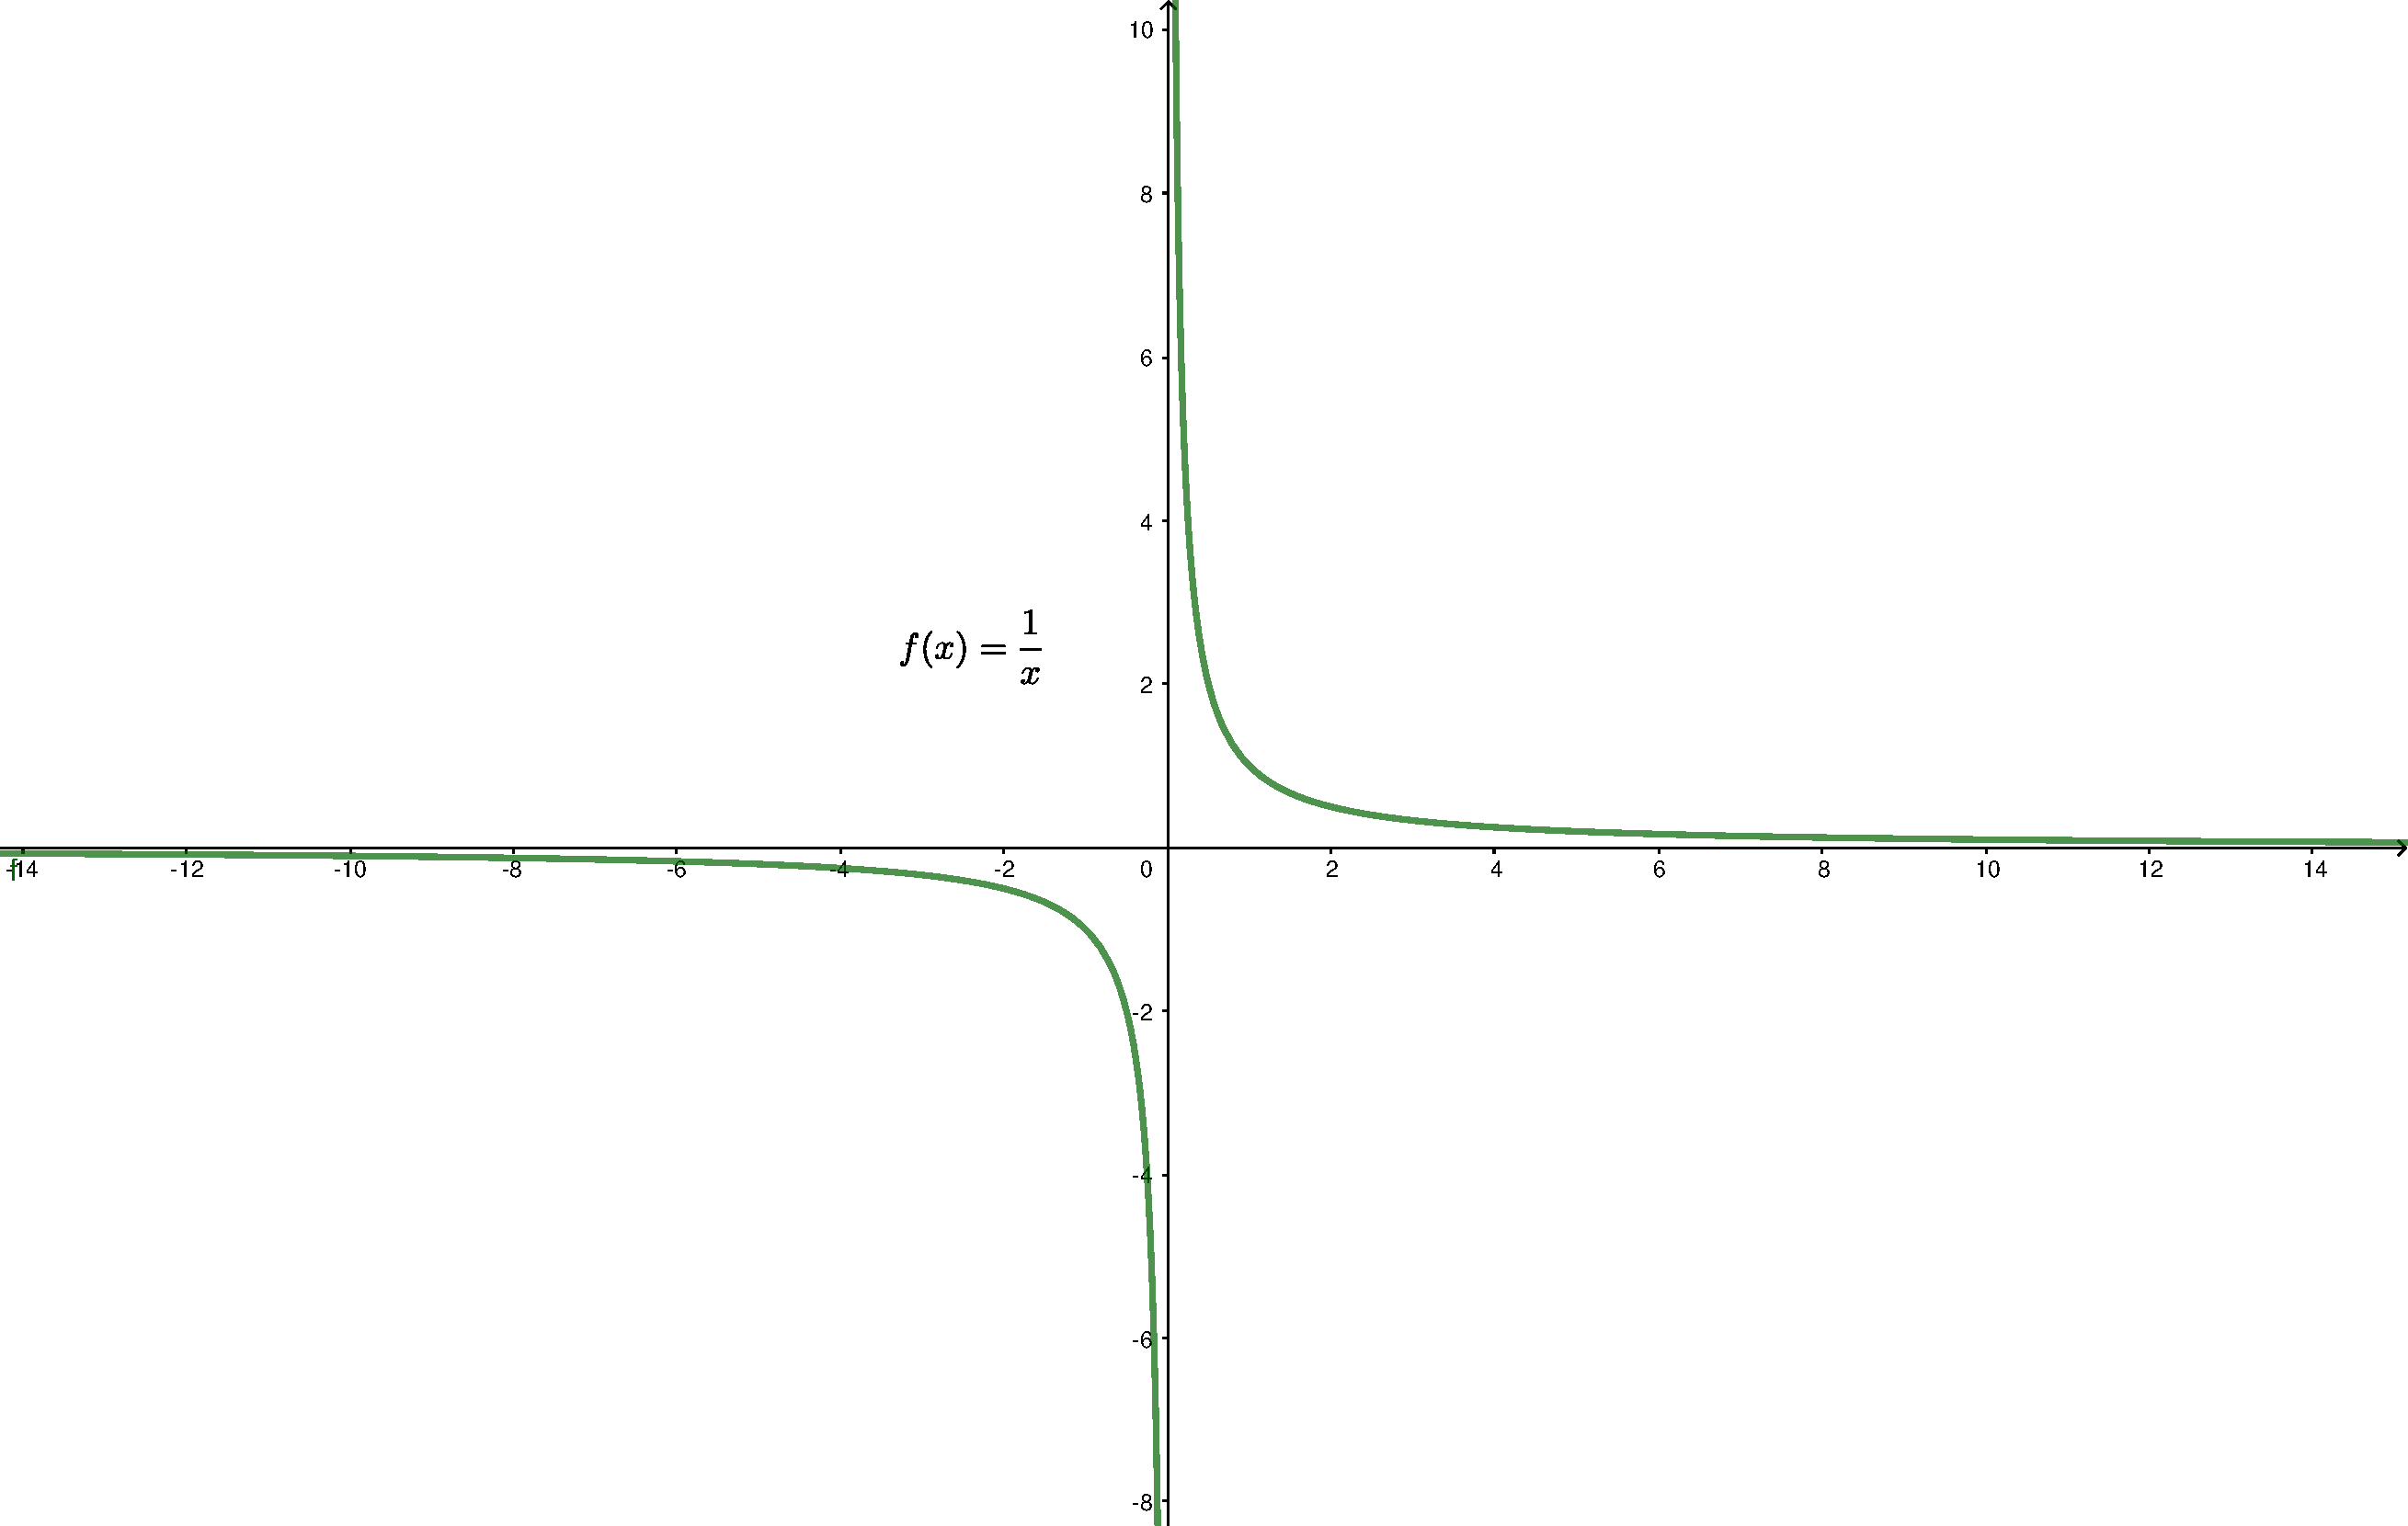
\includegraphics[width=0.7\linewidth]{Figuras/racional}
		\caption{Gráfico da Função Racional $f(x) = \displaystyle \frac{1}{x}$.}
\end{figure}

\subsubsection{Funções Trigonométricas}
\vspace{150pt}
\begin{center}
	\textcolor{red}{FIGURA 15 - REPRESENTAÇÃO GRÁFICA DO CÍRCULO TRIGONOMÉTRICO}
\end{center}

$\sin (\alpha) = \frac{b}{a}$ e $\cos(\alpha) = \frac{c}{a}$

A função seno e a função cosseno são periódicas de período $2\pi$ e satisfazem:
\begin{itemize}
	\item $\sin^{2}(x) + \cos^{2}(x) = 1$;
	\item $\sin(a+b) = \sin(a) \cdot \cos(b) + \sin(b) \cdot \cos(a)$;
	\item $\cos(a+b) = \cos(a) \cdot \cos(b) - \sin(a) \cdot \sin(b)$;
	\item $\sin(x) = - \sin(-x)$ (função ímpar);
	\item $\cos(x) = \cos(-x)$
\end{itemize}


\begin{figure}[!h]
	\centering
	\subfigure[$f(x) = \sin(x)$.]      {\epsfig{figure=sen.pdf,height=6.5cm,width=6.5cm}}
	\subfigure[$f(x) = \cos(x)$.] {\epsfig{figure=cos.pdf,height=6.5cm,width=6.5cm}}
	\caption{Gráfico das Funções Trigonométricas $f(x) = \sin(x)$ e $f(x) = \cos(x)$.}
\end{figure}


Tem-se ainda a função tangente dada por $\tan(x) = \frac{\sin(x)}{\cos(x)}$

\begin{figure}[h!]
	\centering
	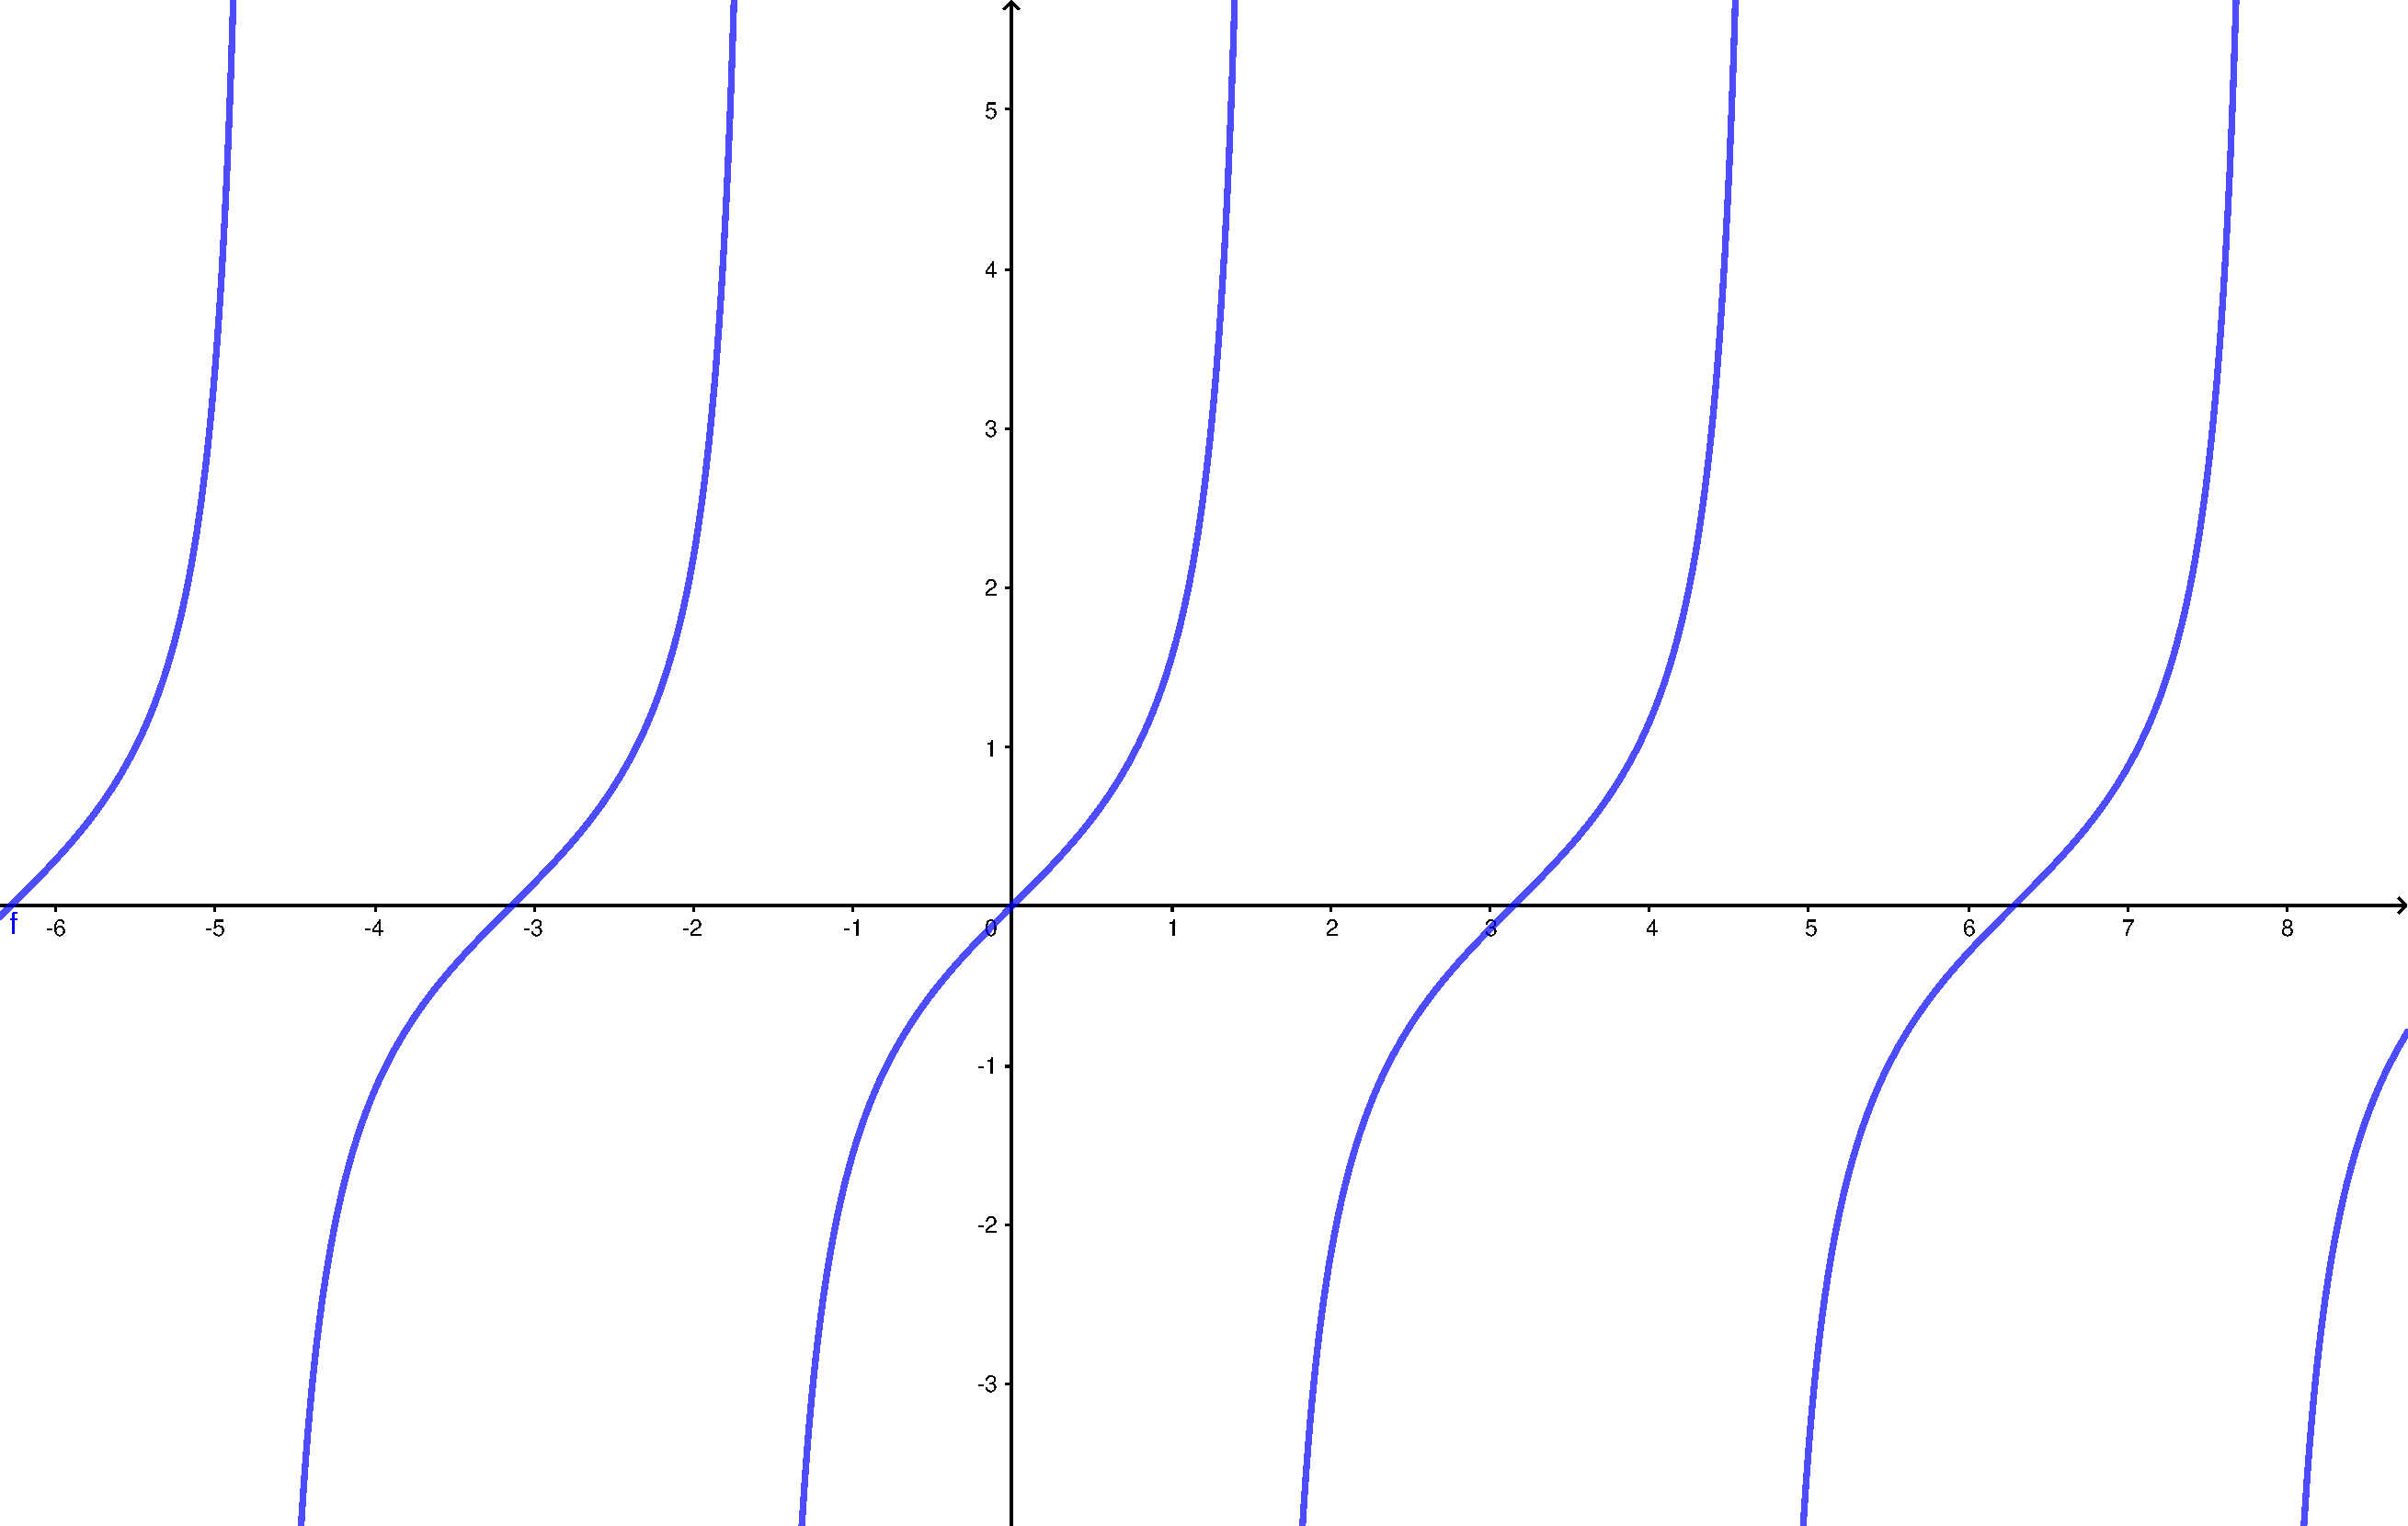
\includegraphics[width=0.7\linewidth]{Figuras/tan}
	\caption{Gráfico da Função Trigonométrica $f(x) = \displaystyle \tan(x)$.}
\end{figure}

\subsubsection{Função Exponencial}

A função exponencial de base $a$ é dada por $f(x) = a^{x}$. Se $x = \frac{p}{q}$ é um número racional, então:
$$a^{\frac{p}{q}} = \sqrt[q]{a^p} = (\sqrt[q]{a})^{p}$$

Consideramos sempre $a>0$ e $a \neq 1$.

\begin{figure}[h!]
	\centering
	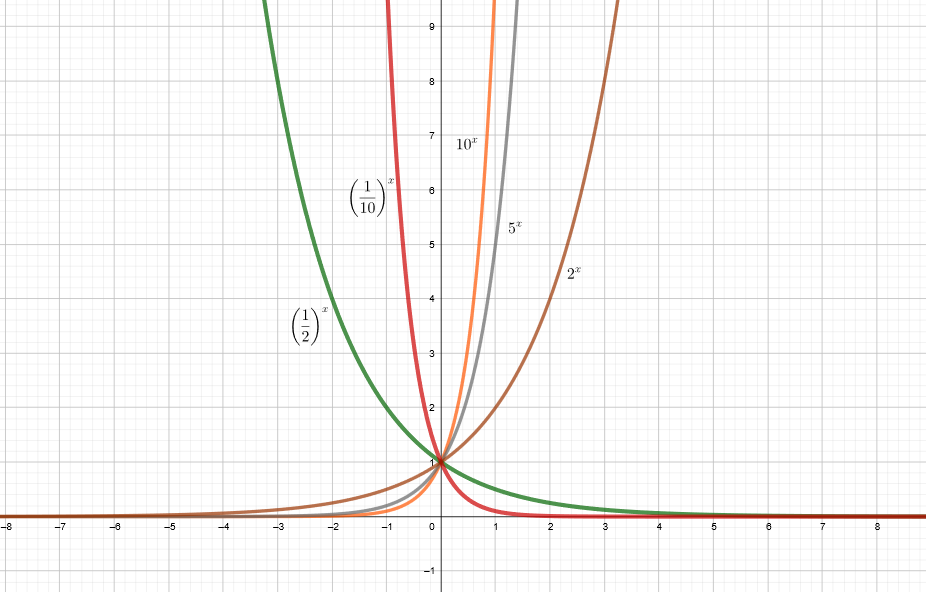
\includegraphics[width=0.8\linewidth]{Figuras/exp}
	\caption{Gráfico das Funções Exponenciais.}
\end{figure}

\newpage

A função exponencial de base $e$, ou seja, $f(x) = e^{x}$, possui coeficiente angulas $1$ quando cruza o eixo $y$.

\begin{figure}[h!]
	\centering
	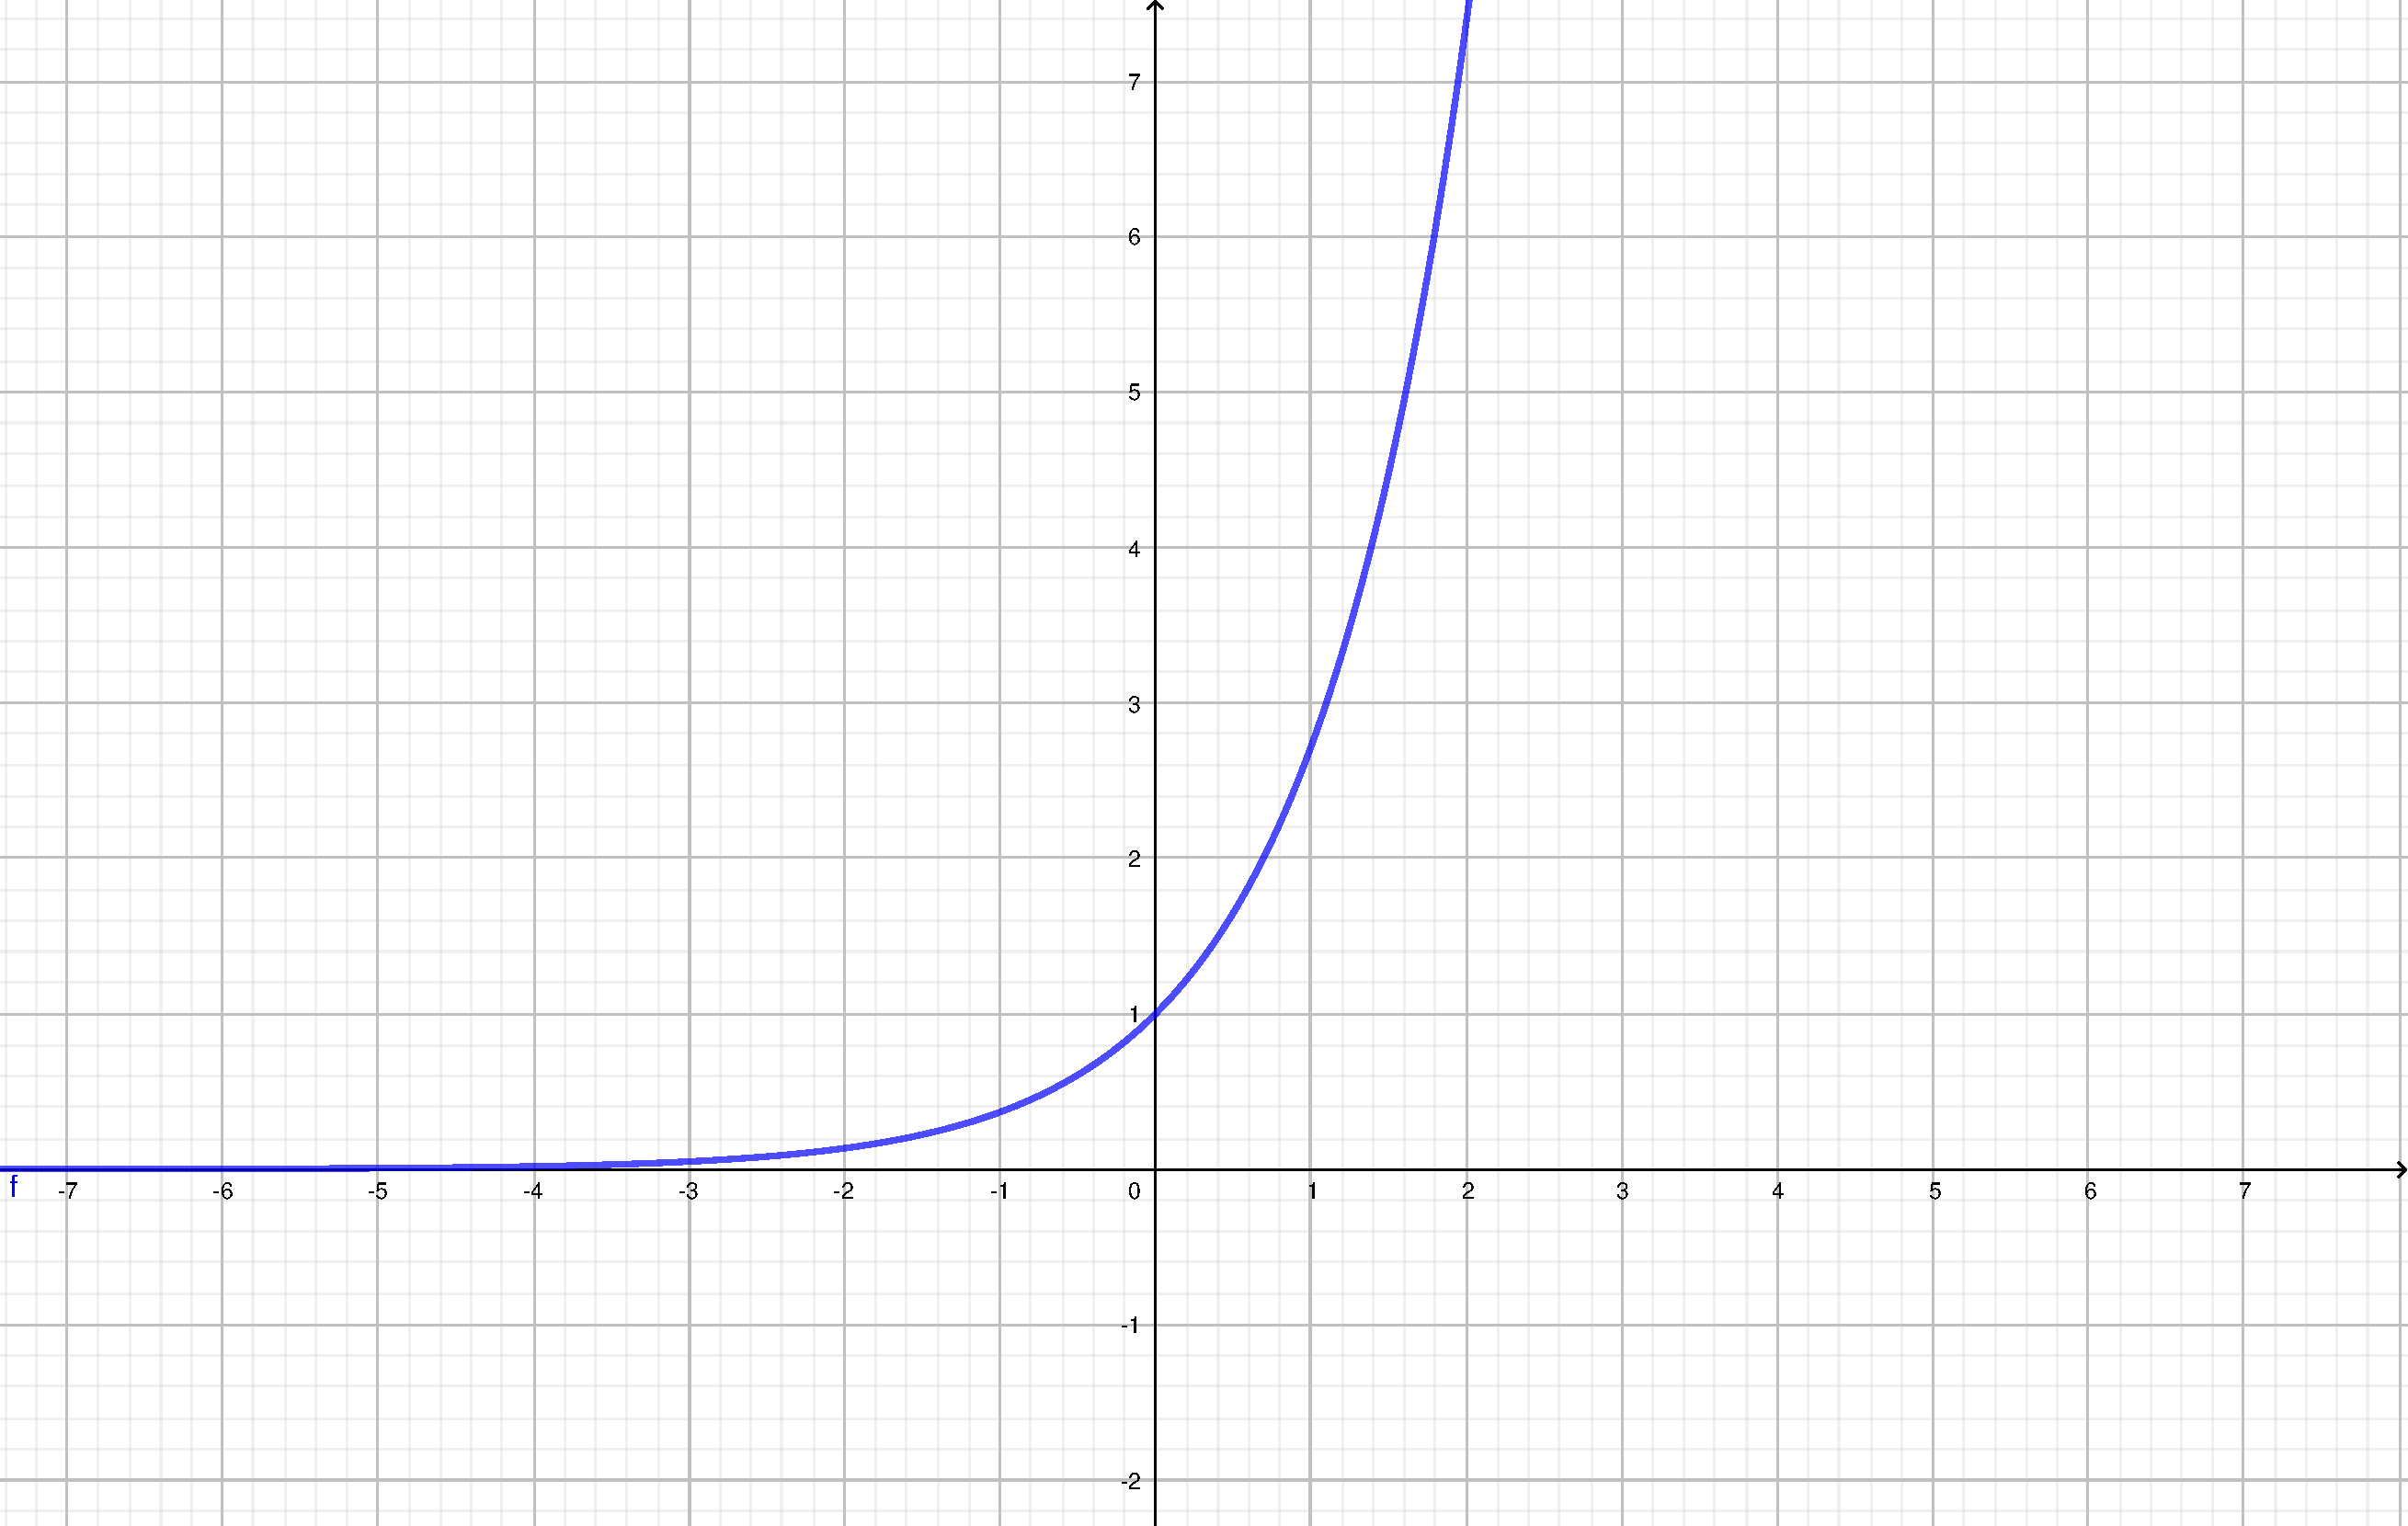
\includegraphics[width=0.8\linewidth]{Figuras/expe}
	\caption{Gráfico das Função Exponencial $f(x) = e^{x}$.}
\end{figure}

\textbf{Algumas propriedades:}
\begin{enumerate}
	\item $a^{x} \cdot a^{y} = a^{x+y}$;
	\item $\frac{a^{x}}{a^{y}} = a^{x-y}$;
	\item $(a^{x})^{y} = a^{xy}$
\end{enumerate}

Além disso, a função $f: \mathbb{R} \rightarrow \mathbb{R}_{+}$ dada por $f(x) = a^{x}$, com $1 \neq a > 0$ é bijetora.


\subsubsection{Função Logarítmica}

A função logarítmica de base $a$ é a inversa da função exponencial de base $a$, ou seja:
$$\log_{a}x = y \Leftrightarrow a^{y} = x$$

Seu domínio é $(0, \infty)$ e sua imagem é $(- \infty, \infty)$

\begin{figure}[h!]
	\centering
	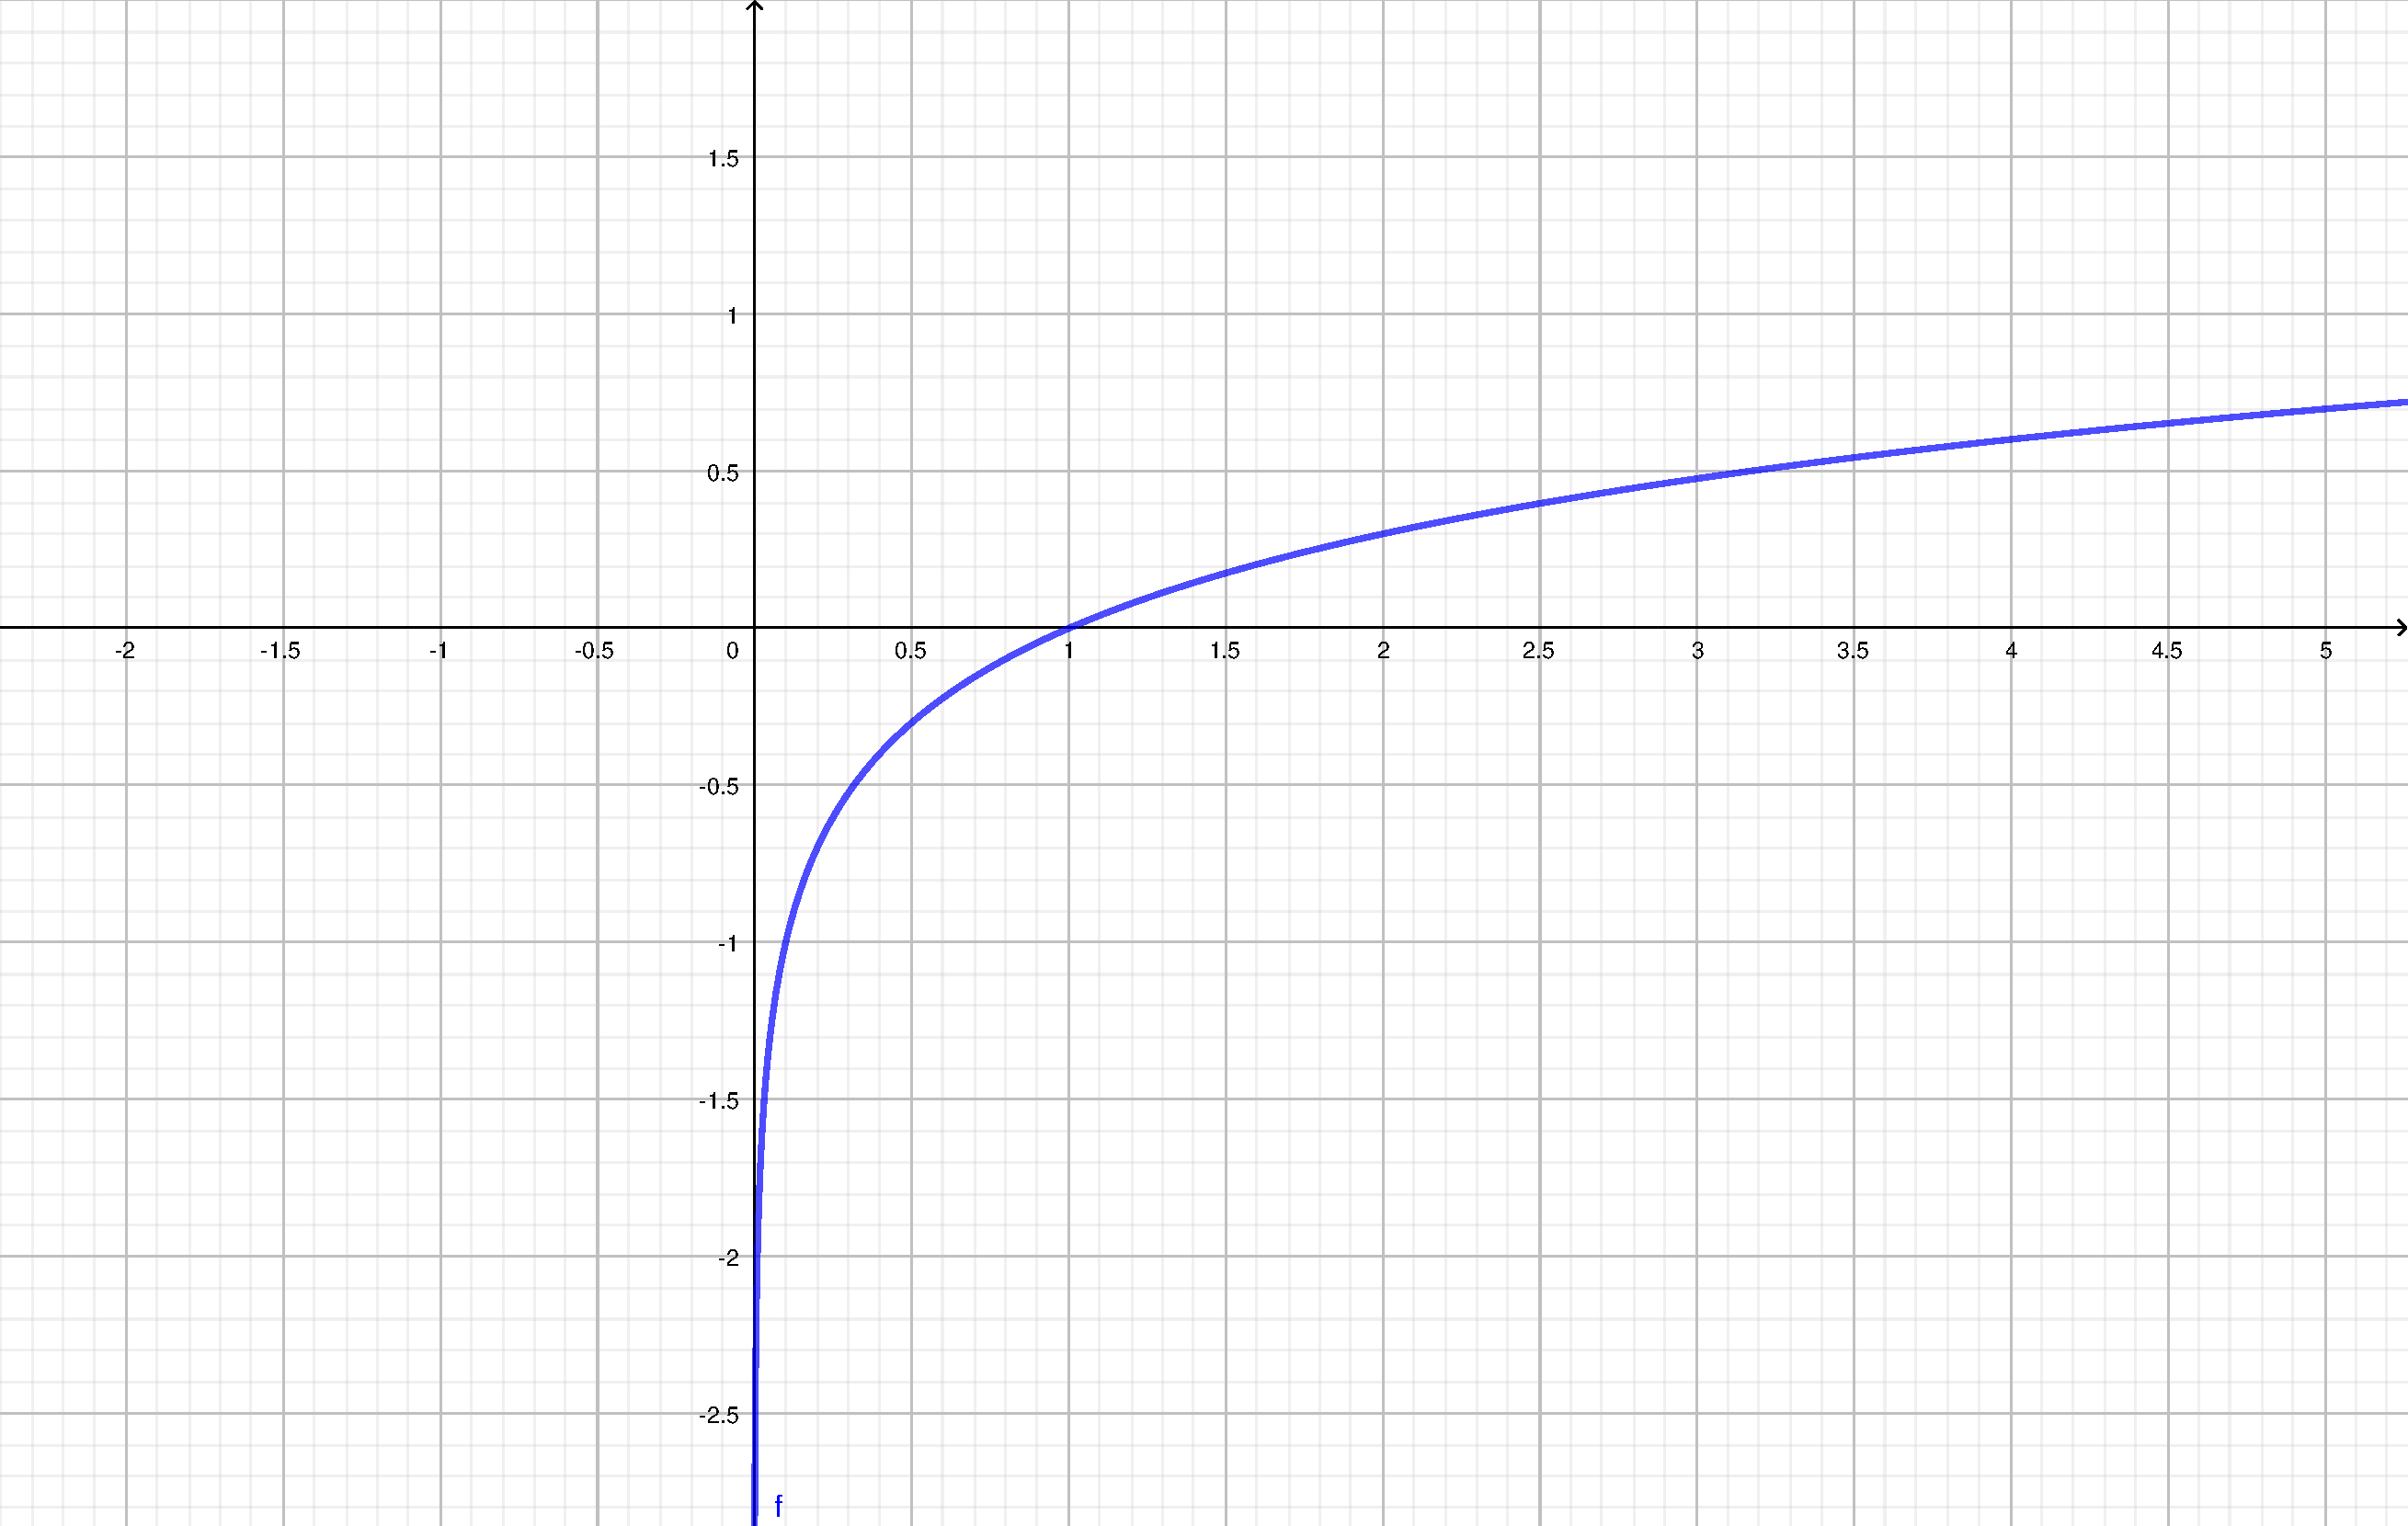
\includegraphics[width=0.8\linewidth]{Figuras/log10}
	\caption{Gráfico das Função Logarítmica $f(x) = \log_{10}x$.}
\end{figure}

Algumas bases recebem notação especial:
$$\log_{a}x = \log(x)$$

$$\log_{e}x = \ln(x)$$

Note que:

$$\ln(x) = y \Leftrightarrow e^{y} = x$$

Assim, qualquer função exponencial pode ser escrita na forma $e^{kx}$, pois
\begin{eqnarray*}
a^{x}	&=& e^{\ln(a^{x})}\\
		&=& e^{x \ln(x)}\\
		&=& e^{kx}
\end{eqnarray*}
Onde $k = \ln(a)$.

Acima utilizamos algumas das seguintes propriedades:
\begin{enumerate}
	\item $\log_{a}(x \cdot z) = \log_{a}x + \log_{a}z$
	\item $\log_{a}(\frac{x}{z}) = \log_{a}x - \log_{a}z$
	\item $\log_{a}(\frac{1}{x}) = - \log_{a}x$
	\item $\log_{a}(x^{z}) = z \log_{a}(x)$
	\item $a^{\log_{a}x} = x$
\end{enumerate}

Note que (mudança de base):
\begin{itemize}
	\item $\log_{b}x = \log_{b}(a^{\log_{a}x})$
	\item $\log_{b}x = \log_{a}x \cdot \log_{b}a$
	\item $\log_{a}x = \frac{\log_{b}x}{\log_{b}a}$
\end{itemize}

Em particular:
$$\log_{a}n = \frac{\ln(n)}{\ln(a)}$$


\newpage
\begin{snugshade}
	\section{Limites e Continuidade}
\end{snugshade}	

Seja $f(x) = \frac{(2x+1)(x-1)}{(x-1)}$ definida em $D_{f} = \{ x \in \mathbb{R}; x \neq 1 \}$. Se $x \neq 1$, então $f(x) = 2x+1$. Mas $f$ não está definida em $x=1$.

\begin{figure}[h!]
	\centering
	\definecolor{ffvvqq}{rgb}{1,0.3333333333333333,0}
	\begin{tikzpicture}[line cap=round,line join=round,>=triangle 45,x=2cm,y=2cm]
	\begin{axis}[
	x=2cm,y=2cm,
	axis lines=middle,
	ymajorgrids=true,
	xmajorgrids=true,
	xmin=-2.5078391442943646,
	xmax=5.523346735472419,
	ymin=-1.1150011120623053,
	ymax=3.977166864209862,
	xtick={-2.5,-2,...,5.5},
	ytick={-1,-0.5,...,3.5},]
	\clip(-2.5078391442943646,-1.1150011120623053) rectangle (5.523346735472419,3.977166864209862);
	\draw[line width=2pt,color=ffvvqq,smooth,samples=100,domain=-2.5078391442943646:5.523346735472419] plot(\x,{((2*(\x)+1)*((\x)-1))/((\x)-1)});
	\begin{small}
	\draw[color=ffvvqq] (-0.9488818215711385,-1.009579817697825) node {$f$};
	\end{small}
	\end{axis}
	\end{tikzpicture}
	\caption{Representação gráfica da função $f(x) = \displaystyle \frac{(2x+1)(x-1)}{(x-1)}$ }
\end{figure}

Podemos dizer que $f(x)$ se aproxima de $3$ se $x$ for suficientemente próximo de 1?

\begin{enumerate}
	\item $|x-1| = 0,1 \Rightarrow |f(x) -3| = 0,2$
	\item $|x-1| = 0,01 \Rightarrow |f(x) -3| = 0,02$
	\item $|x-1| = 0,001 \Rightarrow |f(x) -3| = 0,002$
\end{enumerate}

\begin{table}[h]
	\centering
	\begin{tabular}{|c|c|c|c|}
		\hline
		$x$		&	$0,9$	&	$0,99$		&	$0,999$		\\
		\hline
		$f(x)$	&	$2,8$	&	$2,98$		&	$2,998$		\\
		\hline
		\hline
		$x$		&	$1,1$	&	$1,01$		&	$1,001$		\\
		\hline
		$f(x)$	&	$3,2$	&	$3,02$		&	$3,002$		\\
		\hline
		\hline
				&	$\uparrow 1$	&	$\uparrow 2$	& $\uparrow 3$ 	\\
		\hline 
	\end{tabular}
\end{table}

Se quisermos $|f(x) - 3| < 10^{-6}$, quanto deve ser $x$?

\begin{eqnarray*}
|f(x) -3| < 10^{-6} \\
-10^{-6}	< f(x) - 3	<	10^{-6} \\
-10^{-6}	< 2x+1-3 - 3	<	10^{-6} \\
-10^{-6}	< f(x) - 3	<	10^{-6} \\
-\frac{10^{-6}}{2} < x - 1 < \frac{10^{-6}}{2} 
\end{eqnarray*}

O que resulta em:
$$|x-1| < \frac{10^{-6}}{2} = 5 \cdot 10^{-7}$$

Assim, $|x-1|<5 \cdot 10^{-7}$, $x \neq 1$, implica $|f(x) - 3| < 10^{-6}$.

\begin{definition}[Limites]
	Seja $f(x)$ definida em um intervalo em torno de $a$. Dizemos que o limite de $f(x)$, quando $x$ tende a $a$, é o número $L$, se, para todo $\varepsilon > 0$, existir $\delta > 0$ tal que $|x-a|< \delta$, $x \neq a$, implica em $|f(x)-L|<\varepsilon$. Simbolicamente:
	$$\lim\limits_{x \rightarrow a}f(x) = L \Leftrightarrow \forall \varepsilon > 0, \exists \delta > 0 ; |x-a| < \delta \Rightarrow |f(x) - L| < \varepsilon$$
\end{definition}

No exemplo anterior, dado $\varepsilon > 0$, tome $\delta = \displaystyle \frac{\varepsilon}{2}$ e assim $0 < |x-1| < \delta = \displaystyle \frac{\varepsilon}{2}$ implica em:

{\bf Solução:}
\begin{eqnarray*}
	\left| \displaystyle \frac{(2x+1)(x-1)}{(x-1)} - 3 \right| & = & |2x + 1 -3| \\
	& = & |2(x-1)| \\
	& = & 2|x-1|
\end{eqnarray*}
Como $|x-1| < \displaystyle \frac{\varepsilon}{2}$
\begin{eqnarray*}
	& \implies & 2|x-1| < 2 \displaystyle \frac{\varepsilon}{2} \\
	& \implies & |x-1| < \varepsilon
\end{eqnarray*}

$\therefore \lim\limits_{x \rightarrow 1}f(x) = 3$ onde $f(x) = \displaystyle \frac{(2x+1)(x-1)}{(x-1)}$ $\blacksquare$

{\bf Exemplo:} Seja $f(x) = \begin{cases}
x^2 \text{ , se } x \neq 2 \\
1 \text{ , se } x = 2
\end{cases}
$
prove que $\lim\limits_{x \rightarrow 2}f(x) = 4$

{\bf Solução:}

Dado $\varepsilon > 0$, devemos exibir $\delta > 0$, tal que:
$$0<|x-2|<\delta \implies |x^2 - 4| < \varepsilon$$

{\it Rascunho:}

\begin{eqnarray*}
	|f(x) - 4| < \varepsilon \\
	-\varepsilon < |f(x) - 4| < \varepsilon \\
	-\varepsilon + 4 < |f(x)| < \varepsilon + 4 \\
	-\varepsilon + 4 < |x^2| < \varepsilon + 4\\
	\text{ $x^2$ é sempre positivo} \\
	\sqrt{-\varepsilon + 4} < x < \sqrt{\varepsilon + 4}\\
	\sqrt{-\varepsilon + 4} - 2 < x -2 < \sqrt{\varepsilon + 4} -2\\
	|x-2| < \sqrt{-\varepsilon +4} -2	
\end{eqnarray*}

Tomando $\delta = \min{\{ \sqrt{4 - \varepsilon}-2,\sqrt{4 + \varepsilon}-2\}}>0$

Assim, se $0<|x-2|<\delta$ implica:

\begin{eqnarray*}
	& \sqrt{4 - \varepsilon}-2 \leq -\delta < x - 2< \delta \leq \sqrt{4 + \varepsilon}-2 \\
	& \implies \sqrt{4 - \varepsilon}-2 < x - 2<  \sqrt{4 + \varepsilon}\\
	& \implies \sqrt{4 - \varepsilon} < x <  \sqrt{4 + \varepsilon} \\
	& \implies  4 - \varepsilon < x^2 < 4 + \varepsilon \\
	& \implies  \varepsilon < x^2 -4 < \varepsilon \\
	& \implies  \varepsilon < |f(x) -4| < \varepsilon \\
	& \implies  |f(x) - 4| < \varepsilon
\end{eqnarray*}
\begin{flushright}
	$\blacksquare$
\end{flushright}

Graficamente o limite representa:

\begin{figure}[!h]
	\centering
	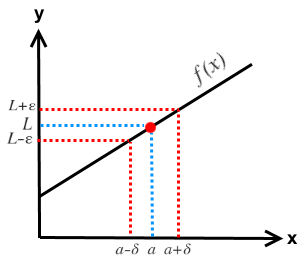
\includegraphics[scale=0.6]{lim}
	\caption{Representação Gráfica - Limite de $f(x)$}
	\label{graflim}
\end{figure}

\begin{theorem}[Unicidade do Limite]
	Se $\lim\limits_{x \rightarrow a}f(x) = L_1$ e $\lim\limits_{x \rightarrow a}f(x) = L_2$, então $L_1 = L_2$
\end{theorem}

\begin{theorem}[Conservação de Sinal]
	Se $\lim\limits_{x \rightarrow a} = L \neq 0$ então existe um intervalo aberto $I$ contendo $a$ tal que, para todo $x \in I \cap D(f)-\{a\}$ tem-se que $f(x)$ possui o mesmo sinal de $L$.
\end{theorem}

\subsection{Propriedades de Limites}
Se $L$, $M$, $a$ e $k$ são números reais e $\lim\limits_{x \rightarrow a}f(x) = L$ e $\lim\limits_{x \rightarrow a}g(x) = M$ são válidas:
\begin{enumerate}
	\item $\lim\limits_{x \rightarrow a}(f(x) + g(x)) = L + M$
	\item $\lim\limits_{x \rightarrow a}(f(x) - g(x)) = L - M$
	\item $\lim\limits_{x \rightarrow a}(f(x) . g(x)) = L . M$
	\item $\lim\limits_{x \rightarrow a}(k.f(x)) = k.L$
	\item $\lim\limits_{x \rightarrow a}\frac{f(x)}{g(x)} = \frac{L}{M}$, desde que $M \neq 0$
	\item $\lim\limits_{x \rightarrow a}(f(x))^{k} = L^k$, se $k \in \mathbb{Z}$
	\item $\lim\limits_{x \rightarrow a}\sqrt[k]{f(x)} = \sqrt[k]{L}$, se $k \in \mathbb{Z}$ e se $L \geq 0$ quando $k$ é par.
\end{enumerate}

{\bf Prova da Propriedade 1}
\newpage

{\bf Exemplo:} Determine $\lim\limits_{x \rightarrow -2}\sqrt{4x^{2}-3}$

\vspace{250pt}

No caso de polinômios temos que $\lim\limits_{x \rightarrow a}P(x) = P(a)$

{\bf Exemplo: } Determine $\lim\limits_{x \rightarrow 1}\frac{x^2+x-2}{x^2-x}$
\vspace{250pt}

{\bf Exemplo: } Determine $\lim\limits_{x \rightarrow 3}\frac{\sqrt{x+1} - 2}{x-3}$
\vspace{250pt}
\newpage

\begin{theorem}
	Se $f(x) \leq g(x)$ para todos os valores de $x$ em certo intervalo aberto contendo $a$, exceto possivelmente no próprio $x=a$, e os limites de $f$ e $g$ existem com $x \rightarrow a$, então:
	$$\lim\limits_{x \rightarrow a}f(x) \leq \lim\limits_{x \rightarrow a}g(x)$$
\end{theorem}

\begin{theorem}[Teorema do Confronto (ou Sanduíche)]
	Se $g(x) \leq f(x) \leq h(x)$ para qualquer $x$ em um intervalo aberto contendo $a$, exceto possivelmente em $x = a$ e $\lim\limits_{x \rightarrow a}g(x) = \lim\limits_{x \rightarrow a}h(x) = L$ então: $\lim\limits_{x \rightarrow a}f(x) = L$
\end{theorem}

{\bf Exemplo: }Temos que $|\sin \theta| < |\theta|$ em uma vizinhança de $\theta = 0$. Mostre que $\lim\limits_{\theta \rightarrow 0}\sin(\theta) = 0$

\vspace{200pt}

Para qualquer função $f(x)$, se $\lim\limits_{x \rightarrow a}|f(x)| = 0$ então $\lim\limits_{x \rightarrow a}f(x) = 0$, pois
\begin{eqnarray*}
|f(x)|  \leq  |f(x)| \\
-|f(x)| \leq  f(x)  \leq |f(x)| 
\end{eqnarray*}

Outra consequência do Teorema do Confronto é a seguinte: se $\lim\limits_{x \rightarrow a}f(x) = 0$ e $|g(x)|<M$ em um intervalo, então $\lim\limits_{x \rightarrow a}f(x).g(x) = 0$.

De fato,
$$|f(x).g(x)| = |f(x)|.|g(x)| \leq |f(x).M|$$
$$ -f(x).M \leq f(x).g(x) \leq f(x).M$$

{\bf Exemplo: } Mostre que $\lim\limits_{x \rightarrow 0}x.\sin(\frac{1}{x}) = 0$

\vspace{200pt}
 
\subsection{Limites Laterais}

\vspace{140pt}
\begin{center}
	\textcolor{red}{FIGURA 21 - REPRESENTAÇÃO GRÁFICA DE LIMITE LATERAL}
\end{center}

Como os dois limites não diferentes, $\lim\limits_{x \rightarrow 1}f(x)$ não existe.

Dizemos que $f(x)$ tem um {\it limite à direita} $L$ em $a$ e escrevemos $\lim\limits_{x \rightarrow a^{+}}f(x)=L$ se 
	$$\lim\limits_{x \rightarrow a^{+}}f(x) = L \Leftrightarrow \forall \varepsilon > 0, \exists \delta > 0 ; a < x < a + \delta \Rightarrow |f(x) - L| < \varepsilon$$

Dizemos que $f(x)$ tem um {\it limite à esquerda} $L$ em $a$ e escrevemos $\lim\limits_{x \rightarrow a^{-}}f(x)=L$ se 
$$\lim\limits_{x \rightarrow a^{-}}f(x) = L \Leftrightarrow \forall \varepsilon > 0, \exists \delta > 0 ; a - \delta < x < a \Rightarrow |f(x) - L| < \varepsilon$$

{\bf Exemplo: } Determine $\lim\limits_{x \rightarrow 0^{+}}\sqrt{x}$
\vspace{200pt}

\begin{theorem}
	Uma função $f(x)$ terá um limite quando $x$ se aproximar de $a$, sendo $f(x)$ definida na vizinhança de $a$, se e somente se, tiver um limite lateral à direita e um à esquerda, e os dois limites laterais forem iguais:
	$$\lim\limits_{x \rightarrow a}f(x) = L \Leftrightarrow \lim\limits_{x \rightarrow a^{-}}f(x) = \lim\limits_{x \rightarrow a^{+}}f(x) = L$$
\end{theorem}

\newpage
{\bf Exemplo: } Determine se existir $\lim\limits_{x \rightarrow 0} = \frac{|x|}{x}$
\vspace{300pt}

{\bf Exemplo: } Determine se existir $\lim\limits_{x \rightarrow 3}f(x)$ onde $f(x) = \begin{cases}
1 - x^2 \text{ , se } x<3 \\
0		\text{ , se } x = 3 \\
x-2		\text{ , se } x >3 
\end{cases}
$


\vspace{350pt}

{\bf Exemplo: } Determine se existir $\lim\limits_{x \rightarrow 1}f(x)$ onde $f(x) = \begin{cases}
2x + 4 \text{ , se } x \leq 1 \\
8x - 2 \text{ , se } x > 1
\end{cases}
$
\vspace{300pt}

\subsection{Limites Fundamentais}
São os seguintes:
\begin{enumerate}
	\item $$\lim\limits_{x \rightarrow 0}\frac{\sin(x)}{x}$$
	\item $$\lim\limits_{x \rightarrow \pm \infty}\left(1 + \frac{1}{x} \right)^{x} = e$$
	\item $$\lim\limits_{x \rightarrow 0}\frac{a^{x}-1}{x} = \ln(a)$$
	\item $$\lim\limits_{x \rightarrow 0}(1+x)^{\frac{1}{x}} = e$$
\end{enumerate}
\newpage
Dedução:
{\bf 1.} 
\newpage

{\bf 2. e 3.}
\newpage

\subsection{Limites Infinitos e Assíntotas}

\vspace{250pt}
\begin{center}
	\textcolor{red}{FIGURA 22 - REPRESENTAÇÃO GRÁFICA DE LIMITE INFINITO}
\end{center}

{\bf Exemplo: } Determine, se existir $\lim\limits_{x \rightarrow 2}\frac{x-3}{x^2-4}$


\vspace{200pt}

\begin{definition}
	Dizemos que $f(x)$ tende ao infinito \emph{ (a menos infinito)} quando $x$ tende a $a$ e escrevemos $\lim\limits_{x \rightarrow a}f(x) = \infty$ \emph{($\lim\limits_{x \rightarrow a}f(x) = - \infty$ )} se para cada número real positivo \emph{(negativo)} $B$ existe um $\delta > 0$ tal que:
	$$0<|x-a|<\delta \Rightarrow f(x) >B $$
	$$0<|x-a|<\delta \Rightarrow f(x) <B $$	
\end{definition}

{\bf Exemplo: } Provar pela definição que $\lim\limits_{x \rightarrow 0}\frac{1}{x^2}=\infty$

\vspace{300pt}

\subsubsection{Assíntotas Verticais}
A reta $x = a$ é uma assíntota vertical do gráfico da função $y = f(x)$ se $\lim\limits_{x \rightarrow a^{+}}f(x) = \pm \infty$ ou $\lim\limits_{x \rightarrow a^{-}}f(x) = \pm \infty$

{\bf Exemplo: } No caso de $y = \sec(x) = \frac{1}{\cos(x)}$ possui infinitas assíntotas verticais onde $\cos(x) = 0$

\vspace{300pt}

A função $\ln(x)$ possui uma assíntota vertical em $x=0$, pois $\lim\limits_{x \rightarrow 0^{+}}\ln(x)= - \infty$

\subsection{Limites no Infinito e Assíntotas}

\begin{definition}
	Dizemos que $f(x)$ possui limite $L$ quando $x$ tende ao infinito \emph{(menos infinito)} e escrevemos $\lim\limits_{x \rightarrow + \infty}f(x) = L$ \emph{($\lim\limits_{x \rightarrow - \infty}f(x) = L$)} se para cada $\varepsilon > 0$, existe um número $M$ tal que:
	$$x > M \Rightarrow |f(x) - L| < \varepsilon$$
	$$x < M \Rightarrow |f(x) - L| < \varepsilon$$
\end{definition}

{\bf OBS. }As regras de limite valem para $x \rightarrow \pm \infty$, incluindo o Teorema do Confronto.

{\bf Exemplo 01: } Determine, se existir $\lim\limits_{x \rightarrow + \infty}\left(5 + \frac{1}{x} \right)$
\vspace{200pt}

{\bf Exemplo 02: } Determine, se existir $\lim\limits_{x \rightarrow \infty}\frac{5x^2+8x-3}{3x^2+2}$
\vspace{200pt}

{\bf Exemplo 03: } Determine, se existir $\lim\limits_{x \rightarrow \infty}\frac{11x+2}{2x^3-1}$
\vspace{200pt}

\begin{definition}
	A reta $y=b$ é uma assíntota horizontal do gráfico da função $y=f(x)$ se $\lim\limits_{x \rightarrow + \infty}f(x) = b$ ou $\lim\limits_{x \rightarrow - \infty}f(x) = b$.
\end{definition}

{\bf Exemplo 01: }$y=0$ é uma assíntota horizontal de $y = e^x$, pois $\lim\limits_{x \rightarrow - \infty}e^x=0$

{\bf Exemplo 02: } Considere $f(x) = 2 + \frac{\sin(x)}{x}$

\vspace{300pt}

{\bf Exemplo 03: } Considere $f(x) = - \frac{8}{x^2-4}$
\vspace{300pt}

\subsubsection{Assíntotas Oblíquas}
{\bf Exemplo: } Considere $f(x) = \frac{2x^2 - 3}{7x + 4}$


\subsection{Continuidade de Funções}


\vspace{250pt}
\begin{center}
	\textcolor{red}{FIGURA 23 - REPRESENTAÇÃO GRÁFICA DE EXEMPLO FUNÇÃO CONTINUA}
\end{center}

Uma função é contínua num ponto interior $c$ de seu domínio quando $\lim\limits_{x \rightarrow c}f(x) = f(c)$

No exemplo em que: $f(x) = \begin{cases}
-x + 1 \text{ ,se } 0 \leq x < 1 \\
2	\text{ ,se } x = 2 \\
x-1 \text{ ,se } 2 < x \leq 3 \\
-x + 5 \text{ ,se } 3 < x \leq 4 \\
1, \text{ ,se } 1 \leq x < 2
\end{cases}
$

$f$ é contínua nos pontos $c \in [0,1) \cup (1,2) \cup (2,4]$ e descontínua nos pontos $c=1$ e $c=2$ pois não existe limite $\lim\limits_{x \rightarrow 1}f(x)$ e, embora $\lim\limits_{x \rightarrow 2}f(x)$ exista, $\lim\limits_{x \rightarrow 2}f(x) = 1 \neq 2 = f(2)$

Assim, $f$ será contínua em $c$ se satisfazer:
\begin{enumerate}
	\item $f(c)$ existe $(c \in D(f))$;
	\item $\lim\limits_{x \rightarrow c}f(x)$ existe, ou seja, $\lim\limits_{x \rightarrow c^{-}}f(x) = \lim\limits_{x \rightarrow c^{+}}f(x)$;
	\item $\lim\limits_{x \rightarrow c}f(x) = f(c)$
\end{enumerate}

{\bf Exemplo: } A função $y = \sin(\frac{2\pi}{x})$ é descontínua na origem, pois $\lim\limits_{x \rightarrow 0}\sin(\frac{2\pi}{x})$ não existe.

\vspace{250pt}
\begin{center}
	\textcolor{red}{FIGURA 23 - REPRESENTAÇÃO GRÁFICA DE $y = \sin(\frac{2\pi}{x})$}
\end{center}

Uma \emph{função contínua} é aquela que é contínua em cada ponto do seu domínio.

{\bf Exemplo: } A função $|x|$ é contínua, pois para $x>0$, $x$ é contínua, para $x<0$, $-x$ também é contínua. Em $x=0$, tem-se $\lim\limits_{x \rightarrow 0}|x| = 0 |0|$.

\begin{theorem}
	Se $f$ e $g$ são contínuas em um ponto $x=c$, então também são contínuas em $x=c$ as seguintes funções:
	\begin{enumerate}
		\item $f+g$;
		\item $f-g$;
		\item $f.g$;
		\item $k.f$ onde $k \in \mathbb{R}$;
		\item $f \circ g$ e $g \circ f$;
		\item $f^{-1}$, se $f$ é bijetora;
		\item $\frac{f}{g}$ se $g(c) \neq 0$;
		\item $\sqrt[r]{f^{s}}$ se $r,s \in \mathbb{Z}$
	\end{enumerate}
\end{theorem}
Como consequência, funções polinomiais e funções racionais são contínuas. Também são contínuas $e^x$, $\ln(x)$, $\sin(x)$ e $\cos(x)$.

\begin{theorem}
	Se $g$ é contínua no ponto $b$ e $\lim\limits_{x \rightarrow a}f(x) = b$, então $\lim\limits_{x \rightarrow a}g(f(x)) = g(b)$, ou seja, $\lim\limits_{x \rightarrow a}g(f(x)) = g(\lim\limits_{x \rightarrow a}f(x))$.
\end{theorem}

{\bf Exemplo 01: }Determine $\lim\limits_{x \rightarrow 1}\sin^{-1}\left(\frac{1-x}{1-x^2}\right)$

\vspace{200pt}

{\bf Exemplo 02: }Determine $\lim\limits_{x \rightarrow 0}\sqrt{x+1}e^{\tan(x)}$

\vspace{200pt}

\subsubsection{Extensão Contínua}

Em alguns casos, podemos estender o domínio de uma função de forma que ela seja contínua nos pontos incluídos no domínio.

{\bf Exemplo: } $f(x) = \frac{\sin(x)}{x}$ não esta definida em $x=0$.

\vspace{200pt}

\begin{theorem}[do Valor Intermediário]
	Seja $y = f(x)$ uma função contínua em um intervalo fechado $[a,b]$. Seja $y_0$ qualquer valor entre $f(a)$ e $f(b)$. Então existe $c \in [a,b]$ tal que $f(c) = y_0$.
\end{theorem}

\vspace{150pt}
\begin{center}
	\textcolor{red}{FIGURA 23 - REPRESENTAÇÃO GRÁFICA DO TEOREMA DO VALOR INTERMEDIÁRIO}
\end{center}

{\bf Exemplo 01: }Discuta as descontinuidades das funções:
\begin{enumerate}
	\item $f(x) = \begin{cases}
	2x+3 \text{ ,se } x \neq 1;\\
	2 \text{ ,se }x = 1
	\end{cases}
	$
	\vspace{200pt}
	\item $f(x) = \frac{1}{x-2}$
	\vspace{200pt}
	\item $f(x) = \begin{cases}
	3x+x \text{ ,se } x \leq 1 \\
	3-x \text{ ,se } x > 1
	\end{cases}
	$
	\vspace{200pt}
\end{enumerate}
\newpage
{\bf Exemplo 02: }Mostre que todo polinômio real de grau ímpar possui ao menos uma raiz real.

\newpage

\section{Derivadas}

\begin{definition}
	Seja $f$ uma função definida em um intervalo aberto $I$ e $x_0$ um elemento de $I$.
	
	A derivada de $f$ no ponto $x_0$ é o limite, se existir:
	\begin{equation}
	\lim\limits_{x \rightarrow x_0}\frac{f(x) - f(x_0)}{x-x_0}
	\end{equation}
	
	Fazendo $x-x_0=h$ tem-se:
	\begin{equation}
	\lim\limits_{x \rightarrow x_0}\frac{f(x) - f(x_0)}{x-x_0} = \lim\limits_{h \rightarrow 0}\frac{f(x_0 + h)-f(x_0)}{h}
	\end{equation}	
	
	{\bf Notação:} $f'(x_0)$ ou $\dfrac{\partial f}{\partial x} |_{x=x_0}$
\end{definition}

\subsection{Interpretação Geométrica}

A derivada nos dá a taxa de variação da função $f$ no ponto $x_0$.

Ou ainda, o coeficiente angular da reta tangente ao gráfico de $f$ no ponto $x=x_0$.

\newpage

{\bf Exemplo:} Calcule a equação da reta tangente e normal a hipérbole $y=\frac{3}{x}$ no ponto $(3,1)$.

\newpage

Se $f$ é uma função derivável em um intervalo, podemos definir a \emph{função derivada} $f'$ que associa a cada $x_0 \in I$ o valor $f'(x_0) = \lim\limits_{x \rightarrow x_0}\frac{f(x) - f(x_0)}{x-x_0}$

{\bf Exemplo:} Calcule a derivada das funções através do conceito de derivada.
\begin{enumerate}
	\item $f(x) = x^2 - 7x + 10$
	\item $f(x) = x^2 + 3x - 7$
	\item $f(x) = \sqrt{x}$
	\item $f(x) = \sqrt[3]{x}$ em $x_0 = 0$
\end{enumerate}
{\bf Exercícios:} 
\begin{enumerate}
	\item Prove que $|x|$ não é derivável em $x_0=0$;
	\item Calcule a derivada de $x|x|$ em $x_0 = 0$;
\end{enumerate}
\newpage

{\bf OBS:} Se $f$ é derivável em $x=x_0$, então $f$ é contínua em $x_0$.

\vspace{230pt}
\subsection{Regras de Derivação}

\begin{enumerate}
	\item {\bf Função Constante:} se $f(x) = c$, então $f'(x) = 0$
	\vspace{150pt}
	\item {\bf Regra da Identidade:} se $f(x) = x$, então $\dfrac{\partial [x]}{\partial x} = 1$
	\vspace{150pt}
	\item {\bf Regra da Potência:} se $f(x) = x^n$, então $\dfrac{\partial [x^n]}{\partial x} = nx^{n-1}$ \\ Exemplo: Determine: \begin{enumerate}
		\item $\dfrac{\partial [x^4]}{\partial x}$
		\item $\dfrac{\partial [\sqrt{x}]}{\partial x}$
		\item $y=\frac{1}{x^2}$
	\end{enumerate}
	\newpage
	\item {\bf  Multiplicação por Constante:} se $w$ é uma função derivável de $x$ e $c$ é uma constante, então $\dfrac{\partial [cw]}{\partial x} = c \dfrac{\partial [w]}{\partial x}$
	\\ Exemplo: Determine: \begin{enumerate}
		\item $\dfrac{\partial [3x^4]}{\partial x}$
		\item $y = 2x^7$
		\item $y = -4x^5$
		\vspace{100pt}
	\end{enumerate}


	\item {\bf Regra da Soma e da Diferença:} $\dfrac{\partial [f(x) \pm g(x)]}{\partial x} = \dfrac{\partial [f(x)]}{\partial x} \pm \dfrac{\partial [g(x)]}{\partial x}$
	\\ Exemplo: Determine: \begin{enumerate}
		\item $y = 3x^4 + 12x$
		\item $y = 7x^5 - 2x^3 + 3x^{-5} = 5x^{\frac{2}{3}} + 2x - 5$
		\vspace{150pt}
	\end{enumerate}


	\item {\bf Derivada da Exponencial:} $\dfrac{\partial [e^x]}{\partial x} = e^x$
	\vspace{150pt}
	
	\item {\bf Regra do Produto:} $\dfrac{\partial [f(x).g(x)]}{\partial x} = f'(x)g(x)+g'(x)f(x)$, generalizando o caso, segue $\dfrac{\partial [u.v]}{\partial x} = u'.v+u.v'$
	\newpage
	Exemplo: Determine: \begin{enumerate}
		\item $y=\frac{1}{x}(x^2 + e^x)$
		\item $y=(x+1)(x^2-3x)$
		\vspace{200pt}
	\end{enumerate}

	\item {\bf Regra do Quociente:}$\dfrac{\partial [\frac{f(x)}{g(x)}]}{\partial x} = \frac{f'(x).g(x) - f(x).g'(x)}{[g(x)]^2}$, generalizando o caso, segue que a derivada é dada por $\dfrac{\partial [\frac{u}{v}]}{\partial x} = \frac{u'.v-u.v'}{[v]^2}$
	\\ Exemplo: Determine: \begin{enumerate}
		\item $y=\frac{x+1}{x-1}$
		\item $y=e^{-x}$
		\item $y=\frac{x^2 - x}{\sqrt{x}}$
		\vspace{230pt}
	\end{enumerate}
\end{enumerate}

\subsection{A Regra da Cadeia}
A Derivada de funções compostas é obtida através da Regra da Cadeia.

\begin{theorem}[Regra da Cadeia]
	Seja $f(x)$ e $g(x)$ tal que $(g \circ f)(x)$ esteja bem definida. Sendo $f(x)$ derivável em $x$ e $g(x)$ derivável em $f(x)$, a derivada de $(g \circ f)(x)$ é:
	\begin{equation}
	(g \circ f(x))' = (g(f(x)))' = g'(f(x)).f'(x)
	\end{equation}
	Na notação de Leibniz, utilizando $u = f(x)$ e $g(f(x))=g(u)$ temos:
	\begin{equation}
	\dfrac{\partial y}{\partial x} = \dfrac{\partial y}{\partial u} . \dfrac{\partial u}{\partial y}
	\end{equation}
\end{theorem}

	{\bf Exemplo:} Determine:
	\begin{enumerate}
		\item $y=(3x^2 + 1)^2$
		\item $y=(x+1)^5$
		\item $y=\sqrt{x+2}$
		\vspace{200pt}
	\end{enumerate}


\subsection{Derivadas das Funções Inversas}
	
\vspace{220pt}
\begin{center}
	\textcolor{red}{FIGURA 23 - REPRESENTAÇÃO DE FUNÇÕES}
\end{center}

\begin{theorem}
	Seja $f$ uma função definida num intervalo aberto $I$. Se $f$ é derivável em $I$ e $f(x) \neq 0$ para todo $x \in I$ então $f$ possui inversa $f^{-1}$ derivável e:
	\begin{equation}
	(f^{-1})' = \frac{1}{f'(f^{-1}(x))}
	\end{equation}
\end{theorem}

A fórmula pode ser obtida através da regra da Cadeia.
\vspace{200pt}

Em outras palavras, seja $a=f^{-1}(b)$ e $b=f(a)$, se $f$ é uma função inversível e derivável no ponto $a = f^{-1}(b)$ sendo $f'(a) \neq 0$, então $(f^{-1})'(b) = \frac{1}{f'(f^{-1}(b))}$

{\bf Exemplo:} $f(x) = x^2$, $x \geq 0$.
\vspace{100pt}

{\bf Exemplo:} $f(x) = x^{3} - 3$ determine $(f^{-1})'$ em $x=6=f(2)$
\vspace{120pt}


\subsection{Derivada de Funções Elementares}

\subsubsection{Derivada da Função Exponencial}
Seja $a \in \mathbb{R}$ tal que $0 < a \neq 1$ e $f(x) = a^x$, então a derivada é: $$y' = a^x .\ln(a)$$

\vspace{200pt}

Caso particular $a = e$, logo $$ y = e^x \Rightarrow y' = e^x .\ln(e) \Rightarrow y' = e^x $$


Generalizando: $$y = a^u \Rightarrow y' = a^u.\ln(a).u'$$ $$y = e^u \Rightarrow y' = e^u.u'$$

{\bf Exemplo:} Calcule a derivada das seguintes funções:
\begin{enumerate}
	\item $y = e^{2x}$
	\item $y = e^{5x}$
	\item $y = e^{-x^2}$
	\item $y = e^{\frac{1}{x}}$
	\item $y = e^{\sqrt{x}}$
	\item $y = xe^{3x}$
	\item $y = \frac{e^{x-1}}{x+2}$
\end{enumerate}
\newpage

\subsubsection{Derivada da Função Logarítmica}
Seja $a \in \mathbb{R}$, tal que $0 < a \neq 1$ e $u(x) = \log_{a}x$ sendo que $f^{-1}(x) = u(x)$ e, $f(x) = a^x$, assim a derivada de $u(x)$ é: $$u'(x) = \frac{1}{f'[f^{-1}(x)]}$$

\vspace{200pt}

Assim, $$u'(x) = \frac{\log_{a}e}{x}$$ $$u' = \frac{1}{x.\ln(a)}$$

No caso particular que $a = e$ segue: $$u' = \frac{1}{x}$$

Generalizando:
$$y = \log_{a}u \Rightarrow y' = \frac{u'}{u.\ln(a)} \text{ ou } y' = \frac{\log_{a}e}{x}$$ 
$$ y = \ln u \Rightarrow y' = \frac{u'}{u}$$

{\bf Exemplo: } Calcule a derivada de 1ª ordem das funções:
\begin{enumerate}
	\item $y = \ln(2x)$
	\item $y = \ln(3x)$
	\item $y = \ln(x^2)$
	\item $y = \ln^2(x)$
	\item $y = \frac{\ln(x)}{x}$
	\item $y = e^x.\ln(1-x)$
	\item $y = e^{\ln(x^2 + x)}$
	\item $y = x^x$
	\item $y = \sqrt{\frac{x+2}{x-1}}$
\end{enumerate}

\vspace{200pt}

\subsubsection{Derivada de Funções Trigonométricas}

{\bf Algumas Relações Trigonométricas}
$$\tan(x) = \frac{\sin(x)}{\cos(x)}$$
$$\cot(x) = \frac{1}{\tan(x)} = \frac{\cos(x)}{\sin(x)}$$
$$cossec(x) = \frac{1}{\sin(x)}$$
$$\sec(x) = \frac{1}{\cos(x)}$$

{\bf Uma Relação Fundamental}
$$\sin^2(x) + \cos^2(x) = 1$$

{\bf Relações Secundárias}
$$\tan^2(x) + 1 = \sec^2(x)$$
$$1 + \cot^2(x) = cossec ^2(x)$$

{\bf Soma do Seno}
$$\sin(a+b) = \sin(a)\cos(b) + \sin(b)\cos(a)$$

As funções $\sin(x)$ e $\cos(x)$ são contínuas e tem derivadas para todo $x$. As derivadas são:
$$\dfrac{\partial [\sin(x)]}{\partial x} = \cos(x)$$
$$\dfrac{\partial [\cos(x)]}{\partial x} = -\sin(x)$$

\newpage

{\bf Exemplos: } Determine a derivada:
\begin{enumerate}
	\item $y = \cot(x)$
	\item $y = \sec(x)$
	\item $y = e^{\cos(x^2 - 3x)}$
	\item $y = \ln(\sin(e^{x^3 - 3x^2}))$
\end{enumerate}
\newpage

\subsubsection{A Função Arco Seno}
Os símbolos $\sin^{-1}(x)$ e $\arcsin(x)$ significam ``um ângulo cujo seno é um dado número $x$''

$$y = \sin (x) \Leftrightarrow y^{-1} = \arcsin(x)$$
$$y = \cos (x) \Leftrightarrow y^{-1} = \arccos(x)$$
$$y = \tan (x) \Leftrightarrow y^{-1} = \arctan(x)$$

Derivadas:
$$(\arcsin[u(x)])' = \frac{1}{\sqrt{1 - u^2}}.u'$$
$$(\arccos[u(x)])' = - \frac{1}{\sqrt{1 - u^2}}.u'$$
$$(\arctan[u(x)])' = \frac{1}{1+u^2}.u'$$

\subsubsection{Funções Hiperbólicas}
São combinações.
$$\sinh(x) = \frac{e^x - e^{-x}}{2}$$
$$\cosh(x) = \frac{e^x +e^{-x}}{2}$$

Derivadas:
$$(\sinh(x))' = \cosh(x)$$
$$(\cosh(x))' = \sinh(x)$$

{\bf Exemplos: } Determine a derivada das funções:
\begin{enumerate}
	\item $f(x) = (\arcsin(x))^2$
	\item $f(x) = \frac{\ln(\sinh(x))}{x}$
	\item $f(x) = sech(\ln(x))$
\end{enumerate}

\subsection{Derivada de Ordem Superior}

Se $y = f(x)$ é uma função derivável, então $f'(x)$ também é uma função. Se $f'$ for derivável teremos $(f')' = f''$ a segunda derivada de $f$.

Notação: $f''(x)$ ou $\dfrac{\partial ^2 f(x)}{\partial x^2}$, generalizando, $f^{n}(x)$ ou $\dfrac{\partial ^{n}f(x)}{\partial x^{n}}$

{\bf Exemplo:} Determine as derivadas de ordem superior das funções:
\begin{enumerate}
	\item $f(x) = x^5 - 3x^4 + 2x^3 - 8x^2 + 10x + 4$
	\item $f(x) = e^x$
	\item $f(x) = \ln(x)$
\end{enumerate}
\newpage

\subsection{Funções Implícitas}

Podemos ter funções na forma explícita:

$y = x^2 + 1$, ou seja, um valor de $y$ para cada $x$

Podemos ter funções na forma implícita:

$x^2 + y^2 = 1$ neste caso, dois valores de $y$ para cada $x$.

Outro exemplos: $x^2 + 1 - e^{xy} = 0$, $\cos(x+y) + 1 - y^2 = 0$, com vários valores de $y = f(x)$

{\bf Exemplo: } Uma função $y = y(x)$ é definida implicitamente pela equação $x^3 + y^3 = 9xy$ e pela condição $y(4) = 2$. Determine a derivada $\dfrac{\partial y(4)}{\partial x}$.

\newpage

{\bf Exemplo: } Calcule a derivada $\dfrac{\partial y(0)}{\partial x}$ implícita da função $xy^{\frac{3}{2}} + 4 = 2x + y$, onde $y(0) = 4$.

\newpage

\subsection{Aplicações de Derivadas}

Uma função $f$ tem um valor mínimo local (máximo local) em um ponto interior $c$ de seu domínio se $f(x) \geq f(c)$ $(f(x) \leq f(c))$ para qualquer $x$ em uma vizinhança de $c$.

\vspace{200pt}

se $f$ possui um valor máximo ou mínimo local em um ponto $c$ interior de seu domínio e se $f$ é derivável em $c$, então $f'(c) = 0$. O contrário não se aplica.

Um ponto interior do domínio de $f$ tal que $f'$ é zero ou indefinida é chamado \emph{ponto crítico} de $f$.

\subsubsection{Teste da Primeira Derivada}

Uma função $f(x)$ é crescente nos intervalos em que $f'(x) > 0$ e é decrescente nos intervalos em que $f'(x) < 0$.
Geometricamente:

\vspace{200pt}

{\bf Exemplo: } Analise:
\begin{enumerate}
	\item $y = 6x + x^2$
	\vspace{250pt}
	\item $y = x^3 - 6x^2 + 9x + 1$
	\vspace{300pt}
\end{enumerate}
\newpage

\subsubsection{Teste da Segunda Derivada}

O sinal da segunda derivada é usado para decidir se um ponto crítico é ponto de máximo ou de mínimo.

\vspace{200pt}

{\bf Exemplo:} Considere $f(x) = -x^2 + 7x - 12$

\vspace{300pt}

\subsection{Teorema do Valor Médio}
\begin{theorem}[de Rolle]
	Se $f$ é uma função contínua em $[a,b]$, derivável em $(a,b)$ e $f(a) = f(b)$, então existe ao menos um ponto $x_0 \in (a,b)$ tal que $f'(x_0) = 0$.
\end{theorem}

\vspace{200pt}

\begin{theorem}[do Valor Médio]
	Se $f$ é uma função contínua em $[a,b]$ e derivável em $(a,b)$ então existe ao menos um ponto $x_0 \in (a,b)$ tal que $f'(x_0) = \frac{f(b) - f(a)}{b-a}$
\end{theorem}

Uma aplicação do Teorema do Valor médio é para mostrar que se a derivada de uma função é nula, então a função é constante.

\vspace{200pt}


\subsection{Regra de L'Hôpital}

Alguns limites mesmo que de funções contínuas, não podem ser resolvidos com a substituição $x=a$ por gerar uma forma indeterminada, tais como: $\frac{0}{0}$, $\frac{\infty}{\infty}$, $\infty - 0$, $\infty - \infty$, $1^{\infty}$, $0^0$ e $\infty^{0}$

\subsubsection{Regra de L'Hôpital}
Sejam $f$ e $g$ funções contínuas e deriváveis em um intervalo aberto $I$ contendo $a$ e suponha que $g'(x) \neq 0$ em $I$, se $x \neq a$ e $f(a) = g(a) = 0$. Então:
$$\lim\limits_{x \rightarrow a}\frac{f(x)}{g(x)} = \lim\limits_{x \rightarrow a}\frac{f'(x)}{g'(x)}$$
desde que o limite do lado direito da igualdade exista.

{\bf Exemplos: } 
\begin{enumerate}
	\item $\lim\limits_{x \rightarrow 0}\frac{\sin(x)}{x}$
	\item $\lim\limits_{x \rightarrow 0}\frac{\cos(x)-1}{x}$
	\item $\lim\limits_{x \rightarrow 0}\frac{\sin(3x)}{\sin(x)}$
\end{enumerate}

{\bf ATENÇÃO:} A Regra de L'Hôpital só pode ser aplicada a limites que resultam em formas indeterminadas.

{\bf Exemplo: } $\lim\limits_{x \rightarrow 0}\frac{\sin(x)}{1+2x}$

\vspace{200pt}

{\bf Exemplos com a forma indeterminada $\frac{\infty}{\infty}$}
\begin{enumerate}
	\item $\lim\limits_{x \rightarrow + \infty}\frac{\ln(x)}{2\sqrt{x}}$
	\vspace{100pt}
	\item $\lim\limits_{x \rightarrow \frac{\pi}{2}}\frac{\sec(x)}{1+\tan(x)}$
	\vspace{100pt}
\end{enumerate}
{\bf Exemplos com a forma indeterminada $0.\infty$}
\begin{enumerate}
	\item $\lim\limits_{x \rightarrow + \infty}x.\sin(\frac{1}{x})$
	\vspace{200pt}
	\item $\lim\limits_{x \rightarrow 0^{+}}\sqrt{x}\ln(x)$
	\vspace{200pt}
\end{enumerate}
{\bf Exemplos com a forma indeterminada $\infty - \infty$}
\begin{enumerate}
	\item $\lim\limits_{x \rightarrow 0^{+}}\left( \frac{1}{\sin(x)} - \frac{1}{x} \right)$
	\vspace{300pt}
	\item $\lim\limits_{x \rightarrow 0^{+}}[cossec(x) - \cot(x) + \cos(x)]$
	\vspace{230pt}
\end{enumerate}
{\bf Exemplos com as formas indeterminadas $1{\infty}$, $0^0$ e $\infty^{0}$}

Nestes casos, aplicamos o logaritmo natural e calculamos $\lim\limits_{x \rightarrow a}\ln(f(x)) = L$, então 
$$\lim\limits_{x \rightarrow a}f(x) = \lim\limits_{x \rightarrow a}e^{\ln(f(x))} = e^{\lim\limits_{x \rightarrow a} \ln(f(x))} = e^L$$

\begin{enumerate}
	\item $\lim\limits_{x \rightarrow 0^{+}}(1+x)^{\frac{1}{x}}$
	\vspace{100pt}
	\item $\lim\limits_{x \rightarrow 0^{+}}x^x$
	\vspace{330pt}
	\item $\lim\limits_{x \rightarrow + \infty}x^{\frac{1}{x}}$
	\vspace{200pt}
\end{enumerate}

\subsection{Linearização de Funções}

\vspace{300pt}

A reta $y = f(a) + f'(a)(x-a)$ é a tangente a $y = f(x)$ no ponto $x = a$.

\vspace{250pt}

Assim, se $f$ é derivável em $x = a$, a função $$L(x) = f(a) + f'(a)(x-a)$$ é denominada \emph{linearização de $f$ em $a$}. O ponto $x = a$ é o \emph{centro} dessa aproximação linear.

{\bf Exemplo: }Vamos aproximar $f(x) = \sqrt{1 + x}$ com centro em $x = 0$.

\newpage

\subsection{Taxas Relacionadas}
São problemas onde as quantidades variáveis estão relacionadas entre sí.

Considere a função composta $h(x) = f(g(x))$.

Pela Regra da Cadeia, $h'(x) = f'(g(x)).g'(x)$ ou $\dfrac{\partial h}{\partial x} = \dfrac{\partial f}{\partial g} . \dfrac{\partial g}{\partial x}$

{\bf Exemplo: } Se uma bolinha de naftalina evapora a uma taxa proporcional à área de sua superfície, mostre que o seu raio decresce a uma taxa constante com o tempo.
\newpage


\section{Integrais}

\subsection{Soma de Riemann}


\vspace{220pt}
\begin{center}
	\textcolor{red}{FIGURA 24 - REPRESENTAÇÃO DA SOMA DE RIEMANN}
\end{center}

\subsection{Integral Definida}
\begin{definition}[Integral Definida]
	Se $f$ é uma função definida em $a \leq x \leq b$, dividimos o intervalo $[a,b]$ em $n$ subintervalos de comprimentos iguais $\Delta x = \frac{(b-a)}{n}$.
	
	Sejam $a = x_0, x_1, x_2, \dots, x_n = b$ os extremos desses subintervalos de forma $x^{*}_i$ está no $i-esimo$ subintervalo $[x_{i-1},x_i]$.
	
	Então a {\bf Integral Definida} em $[a,b]$ é:
	
	$$\int_{a}^{b}f(x)dx = \lim\limits_{n \rightarrow \infty}\sum_{k=1}^{n}f(x_{k}^{*})\Delta x$$
\end{definition}

{\bf Exemplo: } Determine $\int_{0}^{3}(x-1)dx$

\vspace{100pt}

As funções monótonas ou contínuas por partes (incluindo contínuas) são integráveis.

Um exemplo de função não-integrável é:
$$f(x) = \begin{cases}
1, \text{ se } x \in \mathbb{Q} \\
0, \text{ se } x \in \mathbb{R}\backslash\mathbb{Q}
\end{cases}
$$

pois entre $x_k$ e $x_k + \Delta x$ sempre existirá valores em que $f(x_{k}^{*}) = 0$ e $f(x_{k}^{*}) = 1$

$\sum_{k=1}^{n}f(x_{k}^{*})\Delta x = \sum_{k=1}^{n}0.\Delta x  = 0$

$\sum_{k=1}^{n}f(x_{k}^{*})\Delta x = \sum_{k=1}^{n}1.\Delta x = n\Delta x = b -a $

Como o limite das somas de Riemann depende das escolhas de $x_{k}^{*}$, então $f$ não é integrável.

\subsection{Propriedades da Integral Definida}

Ao definirmos $\int_{a}^{b}f(x)dx$, consideramos $a<b$.

Se $b<a$, $\Delta x$ mudará de $\frac{b-a}{n}$ para $\frac{a - b}{n}$. Portanto

$$\int_{b}^{a}f(x)dx = - \int_{a}^{b}f(x)dx$$

Se $a=b$ então $\Delta x = 0$, logo  
$$\int_{a}^{b}f(x)dx = 0$$

{\bf Outras propriedades:}
\begin{enumerate}
	\item $\int_{a}^{b}cdx = c(b-a)$
	\item $\int_{a}^{b}(f(x) \pm g(x))dx = \int_{a}^{b}f(x)dx \pm \int_{a}^{b}g(x)dx$
	\item $\int_{a}^{b}cf(x)dx = c\int_{a}^{b}f(x)dx$
	\item $\int_{a}^{c}f(x)dx + \int_{c}^{b}f(x)dx = \int_{a}^{b}f(x)dx$
\end{enumerate}

{\bf Exemplo: } Suponha que $\int_{-1}^{1}f(x)dx = 5$, $\int_{1}^{4}f(x)dx = 2$ e $\int_{-1}^{1}h(x)dx = 7$. Determine:
$\int_{-1}^{1}[2f(x) + 3h(x)]dx$ e $\int_{-1}^{4}f(x)dx$

\vspace{400pt}

\subsection{Propriedades Comparativas da Integral}

Vamos supor que $a<b$. Então:
\begin{enumerate}
	\item Se $f(x) \geq 0$ para $a \leq x \leq b$, então $\int_{a}^{b}f(x)dx > 0$
	\item Se $f(x) \geq g(x)$ para $a \leq x \leq b$, então $\int_{a}^{b}f(x)dx \geq \int_{a}^{b}g(x)dx$
	\item Se $m \leq f(x) \leq M$ para $a \leq x \leq b$, então
	$m(b-a) \leq \int_{a}^{b}f(x)dx \leq M(b-a)$
\end{enumerate}

{\bf Exemplo: }Mostre que $1 \leq \int_{0}^{1}\sqrt{1 + \cos(x)}dx \leq \sqrt{2}$

\vspace{250pt}

\subsection{Valor Médio de uma Função Contínua}

Seja $f$ uma função contínua não-negativa no intervalo $[a,b]$. Dividindo $[a,b]$ em $n$ subintervalos de larguras $\Delta x = \frac{b-a}{n}$ e calculando $f$ em um ponto $c_k$ de cada intervalo. A média dos $n$ valores amostrados é:
\begin{eqnarray*}
\frac{f(c_1) + f(c_2) + f(c_3) + \dots + f(c_n)}{n} &=& \frac{1}{n}\sum_{k=1}^{n}f(c_k) \\
&=& \frac{\Delta x}{b-a}\sum_{k=1}^{n}f(c_k) \\
&=& \frac{1}{b-a}\sum_{k=1}^{n}f(c_k)\Delta x
\end{eqnarray*}

À medida que aumentamos o tamanho da amostra, a média deve aproximar-se de 
$$\lim\limits_{n \rightarrow \infty}\frac{1}{b-a}\sum_{k=1}^{n}f(c_k)\Delta x = \frac{1}{b-a}\int_{a}^{b}f(x)dx$$


\subsection{Diferenciais}

Seja $y = f(x)$ uma função derivável. A \emph{diferencial $dx$} é uma variável independente. A \emph{diferencial $dy$} é:
$$dy = f'(x)dx$$
Assim, $dy / dx = f'(x) = \frac{dy}{dx}$

{\bf Exemplo: } $\sqrt{1 + x^2}2xdx = \sqrt{u}\dfrac{du}{dx}dx = \sqrt{u}du$

\subsection{O Teorema Fundamental do Cálculo}

Inicialmente, utilizaremos o seguinte lema.

\begin{lemma}
	Se duas funções $f(x)$ e $g(x)$ possuem a mesma derivada $f'(x) = g'(x)$, então elas diferem por uma constante, ou seja, existe $c \in \mathbb{R}$ tal que $f(x) = g(x) + c$
\end{lemma}

{\bf Prova:} Tome $h(x) = f(x) - g(x)$.

Assim, $h'(x) = f'(x) - g'(x) = 0$.

Se $x_1$ e $x_2$ são dois pontos do domínio das funções, então, pelo Teorema do Valor Médio, existe $c$ entre $x_1$ e $x_2$ tal que 
$$\frac{h(x_2) - h(x_1)}{x_2 - x_1} = h'(x) = 0$$

Portanto, dados $x_1$ e $x_2$ quaisquer, $h(x_1) = h(x_2)$. Logo $h(x) = c$, isto é, constante. $\blacksquare$

O Teorema Fundamental do Cálculo nos dará uma relação entre derivadas e integrais.

Seja $f:[a,b] \rightarrow \mathbb{R}$ contínua e $g:[a,b] \rightarrow \mathbb{R}$ definida por $g(x) = \int_{a}^{x}f(t)dt$


\vspace{220pt}
\begin{center}
	\textcolor{red}{FIGURA 25 - REPRESENTAÇÃO DA FUNÇÃO}
\end{center}

$$g(x+h) = \int_{a}^{x+h}f(t)dt$$
$$g(x+h)-g(x) \approx hf(x)$$
$$\frac{g(x+h) - g(x)}{h} \approx f(x)$$

Intuitivamente, se $h \rightarrow 0$, segue
$$\frac{g(x+h) - g(x)}{h} \rightarrow f(x)$$

Logo, $g'(x) = f(x)$.

\begin{theorem}[Fundamental do Cálculo]
	Seja $f$ contínua em $[a,b]$, então:
	\begin{enumerate}
		\item A função $g:[a,b] \rightarrow \mathbb{R}$ definida por $g(x) = \int_{a}^{x}f(t)dt$ $(a \leq x \leq b)$ é contínua em $[a,b]$ e derivável em $(a,b)$ e $g'(x) = F(x)$
		\item Dado $x \in [a,b]$,
		$$\int_{a}^{x}f(t)dt = F(x) - F(a)$$ onde $F$ é qualquer função tal que $F' = f$ ($F$ é primitiva de $f$)
	\end{enumerate}
\end{theorem}

{\bf Prova de 2:} Seja $g(x) = \int_{a}^{x}f(t)dt$, então $g'(x) = f(x)$ para todo $x \in [a,b]$.

Se $F' = f$, então $F(x) = g(x) + c$, para todo $x \in [a,b]$.

Assim,
\begin{eqnarray*}
F(x) - F(a) &=& g(x) + c - (g(a) + c) \\
&=& g(x) - g(a) \\
&=& \int_{a}^{x}f(t)dt - \int_{a}^{a}f(t)dt \\
&=& \int_{a}^{x}f(t)dt, \forall x \in [a,b]
\end{eqnarray*}

$$\int_{a}^{b}f(x)dx = F(b) - F(a)$$ $\blacksquare$

{\bf Notação:} $F(x) |_{a}^{b} = F(b) - F(a)$

{\bf Exemplo:} Calcular a área de um trapézio retângulo por meio do Teorema Fundamental do Cálculo.

\vspace{100pt}

\subsection{Integrais Indefinidas}

O conjunto de todas as primitivas da função é denominado \emph{integral indefinida de $f$ em relação a $x$} e é denotado por 
$$\int f(x)dx$$

Este será representado por uma função (uma primitiva de $f$) mais uma constante arbitrária, considerando que duas primitivas quaisquer de $f$ diferem por uma constante.

{\bf Exemplo: } Determine $\int x^2 dx$

\vspace{300pt}

\subsection{A Regra da Substituição}

Seja $u=g(x)$. Pela regra da cadeia, se $F$ é uma primitiva de $f$, então
$$\dfrac{\partial[F(g(x))]}{\partial x} = f(g(x))g'(x)$$
e
$$\int f(u)du = F(u) + c$$
Logo
$$\int f(g(x))g'(x)dx = \int f(u)du$$

Observe que $g'(x)dx = du$, o que pode ser obtido com:
\begin{eqnarray*}
u & = & g(x) \\
\dfrac{\partial u}{\partial x} & = & g'(x) \\
\partial x g'(x) & = & \partial u
\end{eqnarray*}

{\bf Exemplo 01:} Determine $\int \sqrt{1 + x^2}2x dx$

\vspace{300pt}

{\bf Exemplo 02:} Determine $\int x^2 e^{x^3}dx$

\vspace{300pt}

{\bf Exemplo 03:} Determine $\int_{0}^{\frac{\pi}{4}}\tan(x)dx$
\newpage

{\bf Exemplo 04:} Determine $\int \frac{\ln(x^2)}{x}dx$

\vspace{300pt}

{\bf Exemplo 05:} Determine $\int \frac{2z}{\sqrt[3]{z^2 + 1}}dz$

\vspace{300pt}

\subsection{Fórmula de Substituição na Integral Definida}

$$\int_{a}^{b}f(g(x))g'(x)dx = \int_{g(a)}^{g(b)}f(u)du$$
\vspace{100pt}

{\bf Exemplo: } $\int_{-\frac{\pi}{4}}^{\frac{\pi}{4}}\tan(x)dx$
\newpage

\subsection{Integrais Definidas de Funções Simétricas}

\begin{itemize}
	\item Se $f$ é par, então
	$$\int_{-a}^{a}f(x)dx = 2\int_{0}^{a}f(x)dx$$
	\item Se $f$ é ímpar, então
	$$\int_{-a}^{a}f(x)dx = 0$$
\end{itemize}

{\bf Exemplo:} Determine $\int_{-\frac{\pi}{4}}^{\frac{\pi}{4}}\cos(2x)dx$

\vspace{300pt}

{\bf Exemplo:} Determine $\int_{-\frac{\pi}{4}}^{\frac{\pi}{4}}\sin(2x)dx$

\vspace{100pt}

\subsection{Cálculo de Áreas}

Se $f(x) \geq g(x)$ em $[a,b]$, a área da região entre as curvas $y = f(x)$ e $y = g(x)$ de $a$ até $b$ é a integral de $(f-g)$ desde $a$ até $b$:
$$A = \int_{a}^{b}[f(x)-g(x)]dx$$

\vspace{100pt}
\newpage

{\bf Exemplo 01:}

\vspace{200pt}

{\bf Exemplo 02:} Determine a área da região do primeiro quadrante limitada à esquerda pelo eixo $y$, abaixo pela curva $y =( \frac{x}{2})^2$, acima e à esquerda pela curva $y = \sqrt{x} + 1$ e acima e à direita pela reta $y = -x + 3$

\newpage

\subsection{Funções Transcendentes}
\subsubsection{O Logaritmo definido como uma Integral}

O logaritmo natural de um número positivo $x$ é 
$$\ln(x) = \int_{1}^{x}\frac{1}{t}dt$$

O número $e$ é o número no domínio do logaritmo natural cuja imagem é $1$, ou seja,
$$\ln(e) = \int_{1}^{e}\frac{1}{t}dt = 1$$

\vspace{220pt}
\begin{center}
	\textcolor{red}{FIGURA 26 - REPRESENTAÇÃO DA FUNÇÃO $\ln(x)$}
\end{center}

Pelo Teorema Fundamental do Cálculo, temos $\dfrac{\partial [\ln(x)]}{\partial x} = \dfrac{\partial[\int_{1}^{x}\frac{1}{t}dt]}{\partial x} = \frac{1}{x}$

Como a derivada é sempre positiva, o logaritmo natural é uma função crescente. Logo, é injetora e tem uma inversa.

Ainda, $\dfrac{\partial [\ln(bx)]}{\partial x} = \frac{1}{bx}b = \frac{1}{x}$ onde $b$ é constante qualquer não nula.

Em particular, $\dfrac{\partial [\ln(-x)]}{\partial x} = \frac{1}{x}$

Portanto, para qualquer $x \in \mathbb{R}, x \neq 0$
$$\dfrac{\partial [\ln|x|]}{\partial x} = \frac{1}{x}$$
e
$$\int\frac{1}{u}du = \ln|u| + c$$

{\bf Exemplo: } Determine $\int_{0}^{2}\frac{2x}{x^2 - 5}dx$

\vspace{300pt}

Note que $\ln(2) > \frac{1}{2}$, logo
\begin{eqnarray*}
\ln(2^n) & = & n \ln(2) \\
& > & n \frac{1}{2} \\
& = & \frac{n}{2}
\end{eqnarray*}

Quando $n \rightarrow \infty$, $\frac{n}{2} \rightarrow \infty$, logo $\ln(2^n) \rightarrow \infty$. Ou seja, $\lim\limits_{n \rightarrow \infty}\ln(2^n) = \infty$.

Dado $M > 0$, como $\lim\limits_{n \rightarrow \infty}\ln(2^n) = \infty$ existe $N_1 > 0$ tal que se $n \geq N_1$, implica que $\ln(2^n) > M$. Tome $N = 2^{N_1}$.

Assim, se $x > N \Rightarrow \ln(x) > \ln(N) = \ln(2^{N_1}) > M$

Portanto $\lim\limits_{x \rightarrow + \infty}\ln(x) = \infty$ e analogamente prova-se que $\lim\limits_{x \rightarrow 0^{+}}\ln(x) = -\infty$

Logo $\ln:(0,\infty) \rightarrow (-\infty,+\infty)$ é sobrejetora.

Denotaremos sua inversa por $\ln^{-1}(x)$.

Como $\ln(e^x) = x\ln(e) = x$, segue que $e^x = \ln^{-1}(x)$

A derivada da exponencial assim definida é ela mesma:
\begin{eqnarray*}
\dfrac{\partial e^x}{\partial x} & = & \dfrac{\partial [\ln^{-1}(x)]}{\partial x} \\
& = & \frac{1}{\ln'(\ln^{-1}(x))} \\
& = & \frac{1}{\frac{1}{\ln^{-1}(x)}} \\
& = & \ln^{-1}(x) \\
& = & e^x
\end{eqnarray*}

A função exponencial de base $a$ é definida por
$$a^x = e^{x\ln(a)}$$

A função logaritmo de $x$ com base $a$, ou seja, $\log_{a}x$, é a inversa de $a^x$.

Se $y = \log_{a}x$, então
\begin{eqnarray*}
a^y & = & x \\
\ln(a^y) & = & \ln(x) \\
y\ln(a) & = & \ln(x) \\
y & = & \frac{\ln(x)}{\ln(a)} \\
\log_{a}x & = & \frac{\ln(x)}{\ln(a)}
\end{eqnarray*}
Derivando, temos
\begin{eqnarray*}
\dfrac{\partial [\log_{a}x]}{\partial x} & = & \dfrac{\partial [\frac{\ln(u)}{\ln(a)}]}{\partial x} \\
& = & \frac{1}{\ln(a)}\dfrac{\partial [\ln(u)]}{\partial x} \\
& = & \frac{1}{\ln(a)}\frac{1}{u}\dfrac{\partial u}{\partial x}
\end{eqnarray*}

{\bf Exemplo: } Determine $\int\frac{\log_{2}x}{x}dx$

\vspace{300pt}

\section{Crescimento e Decrescimento Exponencial}

Suponha que uma quantidade $y$ cresça ou decresça a uma taxa proporcional ao seu tamanho, e que a quantidade presente no instante $t = 0$ é $y_0$, então:
$$\begin{cases}
\dfrac{\partial y}{\partial y} = Ky \text{ {\bf Equação Diferencial }} \\
y(0) = y_0 \text{ {\bf Condição Inicial }}
\end{cases}
$$

Disso, segue que:
\begin{eqnarray*}
\frac{1}{y}\dfrac{\partial y}{\partial t} & = & k \\
\int \frac{1}{y}\dfrac{\partial y}{\partial t}dt & = & \int kdt \\
\int \frac{1}{y}dy & = & \int kdt \\
\ln|y| & = & ky + c \\
|y|& = & e^{kt + c} \\
y & = & \pm e^c . e^{kt} \\
y & = & Ae^{kt} 
\end{eqnarray*}
onde $A = \pm e^c$ e $y_0 = y(0) = Ae^{k0} = A$
Portanto
$$y(t) = y_0 e^{kt}$$

\newpage
{\bf Exemplo 01: } Uma colônia de lactobacilos é cultivada sob condições ideais em laboratório, de modo que a população cresce à uma taxa proporcional à população presente. Ao fim de $3$ horas, existem $10000$ bactérias. Ao fim de $5$ horas há $40000$. Quantas bactérias haviam inicialmente?
\newpage

{\bf Exemplo 02: } Pela lei de resfriamento de Newton, se $H$ for a temperatura de um objeto e $H_a$ a temperatura constante do ambiente, então
$$\dfrac{\partial H}{\partial t} = -k(H - H_a)$$
Substituindo $y = H - H_a$
\begin{eqnarray*}
\dfrac{\partial y}{\partial t} & = & \dfrac{\partial H}{\partial t} - \dfrac{\partial H_a}{\partial t} \\
& = & \dfrac{\partial H}{\partial t} \\
& = & -K(H - H_a) \\
& = & -Ky
\end{eqnarray*}
Então, $y(t) = y_0 e^{-kt}$ e assim
$$H - H_a = (H_0 - H_a)e^{-kt}$$
onde $H_0$ é a temperatura inicial.

Se um ovo, a $98^{\circ}$C é colocado para esfriar em um ambiente de $18^{\circ}$C, e depois de $5$min a temperatura do ovo é de $38^{\circ}$C, então, quanto tempo a mais será necessário para que o ovo atinja $20^{\circ}$C?

\newpage

\subsection{Função Hiperbólica}

Toda função definida em um intervalo centrado na origem pode ser escrita como a soma de uma função par e uma função ímpar:
$$f(x) = \underbrace{\frac{f(x)}{2} + \frac{f(-x)}{2}}_{\text{função par}} + \underbrace{\frac{f(x)}{2} - \frac{f(-x)}{2}}_{\text{função ímpar}}$$

Dessa maneira,
$$e^x = \frac{e^x + e^{-x}}{2} + \frac{e^x - e^{-x}}{2}$$

As partes par e ímpar da função exponencial são denominadas cosseno hiperbólico e seno hiperbólico, respectivamente:
$$\cosh(x) = \frac{e^x + e^{-x}}{2}$$
$$\sinh(x) = \frac{e^x - e^{-x}}{2}$$

\subsubsection{Propriedades}
\begin{itemize}
	\item $\cosh^{2}(x) - \sinh^{2}(x) = 1$ \\
	De fato, 
	\begin{eqnarray*}
	\left( \frac{e^x + e^{-x}}{2} \right)^2 - \left( \frac{e^x - e^{-x}}{2} \right)^2 & = & \frac{1}{4}(e^{2x} + 2e^x e^{-x} + e^{-2x} - e^{2x} + 2e^x e^{-x} - e^{-2x}) \\
	& = & 1
	\end{eqnarray*}
	\item $2\sinh(x)\cosh(x) = \sinh(2x)$ \\
	De dato,
	\begin{eqnarray*}
	2 \left( \frac{e^x + e^{-x}}{2} \right) \left( \frac{e^x - e^{-x}}{2} \right) & = & \frac{1}{2}(e^{2x} - e^{-2x}) \\
	& = & \sinh(2x)
	\end{eqnarray*}
\end{itemize}

Em suma, valem as seguintes propriedades:
\begin{enumerate}
	\item $\cosh^2(x) - \sinh^2(x) = 1$ 
	\item $\sinh(2x) = 2\sinh(x)\cosh(x)$
	\item $\cosh(2x) = \cosh^2(x) + \sinh^2(x)$
\end{enumerate}

A propriedade $1$ justifica o nome ``hiperbólico''


\vspace{220pt}
\begin{center}
	\textcolor{red}{FIGURA 27 - REPRESENTAÇÃO DA PROPRIEDADE 1}
\end{center}

Outras funções hiperbólicas básicas:
\begin{itemize}
	\item $\tanh(x) = \frac{\sinh(x)}{\cosh(x)} = \frac{e^x - e^{-x}}{e^x + e^{-x}}$
	\item $\coth(x) = \frac{\cosh(x)}{\sinh(x)} = \frac{e^x + e^{-x}}{e^x - e^{-x}}$
	\item $sech(x) = \frac{1}{\cosh(x)} = \frac{2}{e^x + e^{-x}}$
	\item $cossech(x) = \frac{1}{\sinh(x)} = \frac{2}{e^x - e^{-x}}$	
\end{itemize}

\subsubsection{Derivadas e Integrais}
\begin{itemize}
	\item $\dfrac{\partial [\cosh(x)]}{\partial x} = \sinh(x)$
	\item $\dfrac{\partial [\sinh(x)]}{\partial x} = \cosh(x)$
	\item $\dfrac{\partial [\tanh(x)]}{\partial x} = sech^{2}(x)$	
\end{itemize}

\subsection{Técnicas de Integração}

Por vezes, não é imediato identificar $\int f(g(x))g'(x)dx$ como $\int f(u)du$, mas podemos usar um método algébrico e depois a fórmula da substituição.

\subsubsection{Separando Frações}
$\int \frac{3x + 2}{\sqrt{1-x^2}}dx$

\vspace{400pt}

\subsubsection{Reduzindo uma Fração Imprópria}
$\int \frac{3x^2 - 7x}{3x + 2}dx$

\vspace{400pt}

\subsubsection{Completando o Quadrado}
$\int \frac{1}{\sqrt{8x-x^2}}dx$

\vspace{400pt}

\subsubsection{Usando Identidades Trigonométricas}
$\int_{0}^{\frac{\pi}{4}}\sqrt{a + \cos(4x)}dx$

\vspace{350pt}

\subsubsection{Multiplicando por uma forma de 1}
$\int \sec(x)dx$

\vspace{400pt}

\subsection{Integração por Partes}

Sejam $u$ e $v$ funções deriváveis de $x$. A regra do produto diz que:
\begin{eqnarray*}
(uv)' & = & u'v + uv' \\
\dfrac{\partial [uv]}{\partial x} & = & \dfrac{\partial u}{\partial x}v + \dfrac{\partial v}{\partial x}u \\
\partial[uv] & = & \partial u v + \partial v u \\
uv & = & \int v du + \int u dv \\
\int u dv & = & uv - \int v du
\end{eqnarray*}

Assim, obtemos a fórmula da integração por partes:
$$\int u dv = uv - \int v du$$

{\bf Exemplo 01:} $\int x \cos(x) dx$

\vspace{250pt}

{\bf Exemplo 02:} $\int \ln(x) dx$

\vspace{250pt}

{\bf Exemplo 03:} $\int x^2 e^x dx$

\vspace{400pt}

\subsubsection{Calculando por Partes Integrais Definidas}
{\bf Exemplo 04:} $\int_{0}^{4}xe^{-x}dx$

\vspace{400pt}

{\bf Exemplo 05:} $\int_{0}^{\pi}x^2 \sin(x)dx$

\vspace{320pt}

\subsection{Integração por Frações Parciais}
{\bf Exemplo 01:} $\int \frac{5x-3}{x^2 - 2x -3}dx$

\vspace{400pt}

{\bf Exemplo 02:} $\int \frac{x^2 + 4x + 1}{(x-1)(x+1)(x+3)}dx$

\vspace{330pt}

{\bf Exemplo 03:} $\int \frac{6x + 7}{(x+2)^2}dx$

\vspace{400pt}

{\bf Exemplo 04: (Fator Quadrático Irredutível)} $\int \frac{-2x + 4}{(x^2 + 1)(x-1)^2}dx$

\newpage

{\bf Em resumo:} fatores lineares geram uma fração $\frac{A}{x-a}$.

Fatores lineares repetidos $(x-a)^2$ geram frações $\frac{A}{x-a} + \frac{B}{(x-a)^2}$.

Fatores quadráticos irredutíveis $ax^2 + bx + c$ onde $(b^2 -4ac < 0)$ geram uma função $\frac{Ax + B}{ax^2 + bx + c}$


\subsection{Integrais Trigonométricas} 

$$\sin^{2}(x) + \cos^{2}(x) = 1 $$
$$\sin^{2}(x) = \frac{1 - \cos(2x)}{2}$$
$$\cos^{2}(x) = \frac{1 + \cos(2x)}{2}$$

{\bf Exemplo 01:} $\int \sin^{2}(x)dx$

\vspace{250pt}

{\bf Exemplo 02:} $\int \cos^{5}(x)dx$

\vspace{300pt}

{\bf Exemplo 03:} $\int \sin^{3}(x)\cos^{2}(x)dx$

\vspace{270pt}

{\bf Exemplo 04:} $\int \sin^{2}(x)\cos^{4}(x)dx$

\vspace{500pt}

{\bf Exemplo 05:} $\int \sec^{3}(x)dx$

\vspace{300pt}

\subsubsection{Substituições Trigonométricas}

{\bf Exemplo 01:} $\int \frac{1}{\sqrt{4 + x^2}}dx$

\vspace{300pt}

{\bf Exemplo 02:} $\int \frac{x^2}{\sqrt{9-x^2}}dx$

\vspace{300pt}

{\bf Exemplo 03:} $\int \frac{1}{\sqrt{25x^2 - 4}}$

\vspace{300pt}

{\bf Exemplo 04:} Determine a área da elipse $\frac{x^2}{a^2}+\frac{y^2}{b^2} = 1$

\newpage

\subsection{Equações Diferenciais Separáveis}

Uma equação diferencial de primeira ordem é dita separável se pode ser escrita na forma
$$\dfrac{\partial y}{\partial x} = g(x)h(y)$$
Supondo que $h(y) \neq 0$ para todo $y$, segue que $\dfrac{1}{h(y)}\dfrac{\partial y}{\partial x} = g(x)$, e podemos resolver integrando $\int \frac{1}{h(y)}dy = \int g(x)dx$

Por exemplo, $\dfrac{\partial y}{\partial x} = y^2 x e^{3x+4y}$ é separável, pois equivale a $\dfrac{\partial y}{\partial x} = (xe^{3x})(y^2 e^{4y})$

Mas a equação diferencial ordinal $\dfrac{\partial y}{\partial x} = y + \sin(x)$ não é separável.

{\bf Exemplo:} Resolver o problema de valor inicial
$\begin{cases}
\dfrac{\partial y}{\partial x} = - \frac{x}{y} \\
y(4) = -3
\end{cases}
$

\vspace{300pt}

\subsubsection{Campos de Direções e Curvas Integrais}
A curva $y^2 + x^2 = 25$ é a solução do problema de valor inicial, e $y^2 + x^2 = k$ representa uma família de funções que resolvem a EDO.

\vspace{220pt}
\begin{center}
	\textcolor{red}{FIGURA 28 - REPRESENTAÇÃO DA FAMÍLIA DE FUNÇÕES}
\end{center}

Agora, note que um campo de direções, em um conjunto de pontos $(x,y)$ no plano, pode ser definido por uma EDO $\dfrac{\partial y}{\partial x} = f(x,y)$, onde $\dfrac{\partial y}{\partial x}$ é a inclinação das curvas de nível $y(x)$ no ponto $(x,y)$.

Por exemplo, o campo representado por $\dfrac{\partial y}{\partial x} = - \frac{x}{y}$ possui o seguinte esboço:

\vspace{220pt}
\begin{center}
	\textcolor{red}{FIGURA 29 - REPRESENTAÇÃO DO ESBOÇO}
\end{center}

cujas curvas de nível são dadas pelas soluções da EDO $y^2 + x^2 = k$.


{\bf Exemplo 02:} $\dfrac{\partial y}{\partial x} = (1 + y^2)e^x$

\vspace{200pt}

{\bf Exemplo 03:} $y' = y^2x^3$

\vspace{300pt}

\subsection{Integrais Impróprias}

Vamos atribuir um valor para a área abaixo da curva $y = e^{-\frac{x}{2}}$, $x>0$.

\vspace{220pt}
\begin{center}
	\textcolor{red}{FIGURA 30 - REPRESENTAÇÃO DA FUNÇÃO $y = e^{-\frac{x}{2}}$, $x>0$ }
\end{center}

Primeiro, calculamos a área para $x$ variando de $0$ até $b$, e depois calculamos o seu limite quando $b \rightarrow \infty$.

\begin{eqnarray*}
A(b) & = & \int_{0}^{b}e^{-\frac{x}{2}}dx \\
& = & [-2e^{-\frac{x}{2}}]|_{0}^{b} \\
& = & -2(e^{-\frac{b}{2}}-1) 
\end{eqnarray*}

Daí,
\begin{eqnarray*}
\lim\limits_{b \rightarrow \infty}A(b) & = & \lim\limits_{b \rightarrow \infty}(-2(e^{-\frac{b}{2}}-1)) \\
& = & (-2 (0-1)) \\
& = & 2
\end{eqnarray*}

Podemos escrever:
$$\int_{0}^{\infty}e^{-\frac{x}{2}}dx = \lim\limits_{b \rightarrow \infty}\int_{0}^{b}e^{-\frac{x}{2}}dx$$

Generalizando,
$$\int_{a}^{\infty}f(x)dx = \lim\limits_{b \rightarrow \infty}\int_{a}^{b}f(x)dx$$

$$\int_{-\infty}^{b}f(x)dx = \lim\limits_{a \rightarrow - \infty}\int_{a}^{b}f(x)dx$$

Se o limite existe (finito), dizemos que a integral \emph{converge}, caso contrário, dizemos que ela \emph{diverge}.

{\bf Exemplo 01:} $\int_{1}^{\infty}\frac{\ln(x)}{x^2}dx$
\vspace{300pt}

{\bf Exemplo 02:} $\int_{-\infty}^{\infty}\frac{1}{1+x^2}dx$

\vspace{300pt}

Outro tipo de integral imprópria aparece quando o integrando tem uma assíntota vertical.

Por exemplo, $\int_{0}^{1}\frac{1}{x^2}dx$


\vspace{200pt}
\begin{center}
	\textcolor{red}{FIGURA 31 - REPRESENTAÇÃO DA FUNÇÃO $y = \frac{1}{x^2}$ }
\end{center}

Neste caso, calculamos a integral $\int_{a}^{1}\frac{1}{x^2}dx$ e fazemos $a \rightarrow 0^{+}$

\begin{eqnarray*}
\int_{0}^{1}\frac{1}{x^2}dx & = & - \frac{1}{x}|_{0}^{1} \\
& = & -1 - \lim\limits_{a \rightarrow 0^{+}} \left( - \frac{1}{a} \right) \\
& = & -1 - (- \infty) \\
& = & \infty
\end{eqnarray*}

Ou seja, a integral diverge.

{\bf Exemplo:} $\int_{0}^{1}\frac{1}{\sqrt{x}}dx$

\vspace{180pt}

{\bf Exemplo:} $\int_{0}^{1}\frac{1}{(x-1)^{\frac{2}{3}}}dx$
\vspace{180pt}

{\bf Exemplo:} $\int_{0}^{3}\frac{1}{x-1}dx$
\vspace{350pt}

\subsubsection{Testes para Convergência e Divergência}
\begin{itemize}
	\item $$\int_{1}^{\infty}\frac{1}{x^p}dx \Rightarrow \begin{cases}
		\text{ converge, se }p > 1 \\
		\text{ diverge, se } p \leq 1
	\end{cases}$$
	\item $$ \int_{1}^{\infty}a^x dx \Rightarrow \begin{cases}
	\text{ converge, se } a < 1 \\
	\text{ diverge, se } a \geq 1
	\end{cases}$$
\end{itemize}

{\bf Teste da Comparação:} sejam $f$ e $g$ contínuas em $[a,\infty)$, com $0 \leq f(x) \leq g(x) $ para qualquer $x \geq a$. Então:
\begin{enumerate}
	\item $\int_{a}^{\infty}f(x)dx$ converge se $\int_{a}^{\infty}g(x)dx$ converge;
	\item $\int_{a}^{\infty}g(x)dx$ diverge se $\int_{a}^{\infty}f(x)dx$ diverge.
\end{enumerate}

{\bf Exemplo:} $\int_{1}^{\infty}\frac{\sin^{2}(x)}{x^2}dx$ converge.

\vspace{200pt}

{\bf Exemplo:} $- \int_{1}^{\infty}\frac{1}{\sqrt{x^2 - 2}}dx$ diverge.

\vspace{300pt}

{\bf Teste da Comparação no Limite:} se $f$ e $g$ são funções positivas contínuas em $[a,\infty)$ e se
$$\lim\limits_{x \rightarrow \infty}\frac{f(x)}{g(x)} = L, \text{   } 0 < L < \infty$$
então $\int_{a}^{\infty}f(x)dx$ e $\int_{a}^{\infty}g(x)dx$ são ambas convergentes ou ambas divergentes.

{\bf Exemplo:} As funções $f(x) = \frac{1}{x^2}$ e $g(x) = \frac{1}{1 + x^2}$ são positivas e contínuas em $[1,\infty)$. Além disso:
\begin{eqnarray*}
\lim\limits_{x \rightarrow \infty}\frac{f(x)}{g(x)} & = & \lim\limits_{x \rightarrow \infty}\frac{\frac{1}{x^2}}{\frac{1}{x^2 + 1}} \\
& = & \lim\limits_{x \rightarrow \infty}\frac{1 + x^2}{x^2} \\
& = & \lim\limits_{x \rightarrow \infty}\frac{2x}{2x} \\
& = & 1
\end{eqnarray*}

Consequentemente, $\int_{1}^{\infty}\frac{1}{1+x^2}dx$ converge porque $\int_{1}^{\infty}\frac{1}{x^2}dx$ converge.

Entretanto, elas convergem para valores diferentes:
\begin{eqnarray*}
\int_{1}^{\infty}\frac{1}{x^2}dx & = & \left .-\frac{1}{x}\right|^{\infty}_{1} \\
& = & \lim\limits_{x \rightarrow \infty}\left( - \frac{1}{x} \right) - \left( - \frac{1}{1} \right) \\
& = & 1
\end{eqnarray*}

\begin{eqnarray*}
\int_{1}^{\infty}\frac{1}{x^2 + 1}dx & = & \arctan(x) |_{1}^{\infty} \\
& = & \lim\limits_{x \rightarrow \infty} \arctan(x) - \arctan(1) \\
& = & \frac{\pi}{2} - \frac{\pi}{4} \\
& = & \frac{\pi}{4}
\end{eqnarray*}

{\bf Exemplo 02:} Mostrar que $\int_{1}^{\infty}\frac{3}{e^x + 5}dx$ converge.

\vspace{300pt}


\newpage
\begin{center}
{\Large{\bf Tabela de Integrais}}	
\end{center}

%\begin{multicols}{2}
	\begin{enumerate}
		\item $\displaystyle \int cdx = cx + k$
		\item $\displaystyle \int x^{\alpha}dx = \frac{x^{\alpha + 1}}{\alpha + 1} + k$, $\alpha \neq -1$
		\item $\displaystyle \int e^x dx = e^x + k$
		\item $\displaystyle \int \frac{1}{x}dx = \ln(x) + k$, $(x > 0)$
		\item $\displaystyle \int \frac{1}{x}dx = \ln(-x) + k$, $(x < 0)$
		\item $\displaystyle \int \frac{1}{x}dx = \ln|x| + k$
		\item $\displaystyle \int \sin(x) dx = - \cos(x) + k$
		\item $\displaystyle \int \cos(x) dx = \sin(x) + k$
		\item $\displaystyle \int \sec^{2}(x)dx = \tan(x) + k$
		\item $\displaystyle \int \sec(x).\tan(x)dx = \sec(x) + k$
		\item $\displaystyle \int \sec(x)dx = \ln|\sec(x)+\tan(x)| + k$
		\item $\displaystyle \int \tan(x)dx = -\ln|\cos(x)|+ k$
		\item $\displaystyle \int \frac{1}{1+x^2}dx = \arctan(x) + k$
		\item $\displaystyle \int \frac{1}{\sqrt{1 - x^2}}dx = \arcsin(x) + k$
		\item $\displaystyle \int \tan^{n}(x)\sec^{2}(x)dx = \tan^{n+1}(x) + k$, $(n \neq -1)$
		\item $\displaystyle \int \sec^{n}(x)\sec(x)\tan(x)dx = \sec^{n+1}(x) + k$, $(n \neq -1)$
		\item $\displaystyle \int \tan^{n}(x)dx = \tan^{n-1}(x) - \displaystyle \int \tan^{n-2}(x)dx$
		\item $\displaystyle \int \sec^{n}(x)dx = \sen^{n-2}(x)\tan(x) + \frac{n-2}{n-1}\displaystyle \int \sec^{n-2}(x)dx$
	\end{enumerate}
%\end{multicols}


\newpage

{\bf Exercício:} Qual o valor da expressão?
$$\left[(3^{0,3333333})^{27}+ 2^{2^1} - \sqrt[5]{239 + \sqrt[3]{\frac{448}{7}}}-(\sqrt[3]{3})^{3^3} \right]^{\sqrt[7]{92}}$$
{\bf Resolução:}\\
$$\left[(3^{\frac{3}{9}})^{27}+ 2^2 - \sqrt[5]{239 + \sqrt[3]{64}}-(\sqrt[3]{3})^{27} \right]^{\sqrt[7]{92}}$$
$$\left[4 - \sqrt[5]{239 + 4}\right]^{\sqrt[7]{92}}$$
$$\left[4 - \sqrt[5]{3^5}\right]^{\sqrt[7]{92}}$$
$$\left[4 - 3\right]^{\sqrt[7]{92}}$$
$$1$$

\rule{17cm}{0.7mm}

\end{document}
